%% This is file `DEMO-TUDaThesis.tex' version 3.28 (2022/11/15),
%% it is part of
%% TUDa-CI -- Corporate Design for TU Darmstadt
%% ----------------------------------------------------------------------------
%%
%%  Copyright (C) 2018--2022 by Marei Peischl <marei@peitex.de>
%%
%% ============================================================================
%% This work may be distributed and/or modified under the
%% conditions of the LaTeX Project Public License, either version 1.3c
%% of this license or (at your option) any later version.
%% The latest version of this license is in
%% http://www.latex-project.org/lppl.txt
%% and version 1.3c or later is part of all distributions of LaTeX
%% version 2008/05/04 or later.
%%
%% This work has the LPPL maintenance status `maintained'.
%%
%% The Current Maintainers of this work are
%%   Marei Peischl <tuda-ci@peitex.de>
%%   Markus Lazanowski <latex@ce.tu-darmstadt.de>
%%
%% The development respository can be found at
%% https://github.com/tudace/tuda_latex_templates
%% Please use the issue tracker for feedback!
%%
%% If you need a compiled version of this document, have a look at
%% http://mirror.ctan.org/macros/latex/contrib/tuda-ci/doc
%% or at the documentation directory of this package (if installed)
%% <path to your LaTeX distribution>/doc/latex/tuda-ci
%% ============================================================================
%%
% !TeX program = lualatex
%%

\documentclass[
	ngerman,
	ruledheaders=section,%Ebene bis zu der die Überschriften mit Linien abgetrennt werden, vgl. DEMO-TUDaPub
	class=report,% Basisdokumentenklasse. Wählt die Korrespondierende KOMA-Script Klasse
	thesis={type=master},% Dokumententyp Thesis, für Dissertationen siehe die Demo-Datei DEMO-TUDaPhd
	accentcolor=1d,% Auswahl der Akzentfarbe
	custommargins=true,% Ränder werden mithilfe von typearea automatisch berechnet
	marginpar=false,% Kopfzeile und Fußzeile erstrecken sich nicht über die Randnotizspalte
	%BCOR=5mm,%Bindekorrektur, falls notwendig
	parskip=half-,%Absatzkennzeichnung durch Abstand vgl. KOMA-Script
	fontsize=11pt,%Basisschriftgröße laut Corporate Design ist mit 9pt häufig zu klein
%	logofile=example-image, %Falls die Logo Dateien nicht vorliegen
]{tudapub}


% Der folgende Block ist nur bei pdfTeX auf Versionen vor April 2018 notwendig
%\usepackage{iftex}
%\ifPDFTeX
%	\usepackage[utf8]{inputenc}%kompatibilität mit TeX Versionen vor April 2018
%\fi

%%%%%%%%%%%%%%%%%%%
%Sprachanpassung & Verbesserte Trennregeln
%%%%%%%%%%%%%%%%%%%
\usepackage[ngerman, main=english]{babel}
\usepackage{microtype}
\usepackage{xcolor}
\usepackage{tikz}
\usetikzlibrary{automata, positioning, arrows.meta, shapes.geometric, calc, backgrounds}
\usepackage{amssymb}
\usepackage{stmaryrd}
\usepackage{booktabs} 
\usepackage{tabularx} 
\usepackage{threeparttable}

\usepackage{dsfont}


%Paket für Code Listings
%\usepackage[T1]{fontenc}
\usepackage[newfloat]{minted}
\setminted{
	linenos=true,             % Zeilennummern aktivieren
	numbersep=5pt,            % Abstand der Nummern zum Code
	xleftmargin=15pt,         % Einrückung, damit Nummern nicht über den Rand ragen
	fontsize=\footnotesize,   % Schriftgröße verkleinern
	framesep=2mm,
	breaklines=true,          % Automatischer Zeilenumbruch
	tabsize=2                 % Tabulator-Breite
}
\usepackage[most]{tcolorbox}
\tcbuselibrary{minted}


\usepackage[autostyle]{csquotes}% Anführungszeichen vereinfacht


%%%%%%%%%%%%%%%%%%%
%Literaturverzeichnis
%%%%%%%%%%%%%%%%%%%
\usepackage[
backend=biber,
style=numeric,
doi=false,
url=true
]{biblatex}
% Literaturverzeichnis
\addbibresource{DEMO-TUDaBibliography.bib}
\usepackage{hyperref}
\hypersetup{
	colorlinks=true,
	citecolor=blue,
	linkcolor=blue,
	urlcolor=blue
}



% Für Hintergrundfarben
\usepackage{caption} % Für schöne Bildunterschriften


\usepackage{subcaption}

%\usepackage{cite}






%Formatierungen für Beispiele in diesem Dokument. Im Allgemeinen nicht notwendig!
\let\file\texttt
\let\code\texttt
\let\tbs\textbackslash
\let\pck\textsf
\let\cls\textsf

\usepackage{pifont}% Zapf-Dingbats Symbole



\usepackage[english, capitalise, noabbrev]{cleveref}


%%%%%%%%%%%%%%%%%%%
%Paketvorschläge Mathematik
%%%%%%%%%%%%%%%%%%%
%\usepackage{mathtools} % erweiterte Fassung von amsmath
%\usepackage{amssymb}   % erweiterter Zeichensatz
%\usepackage{siunitx}   % Einheiten


\newcommand*{\FeatureTrue}{\ding{52}}
\newcommand*{\FeatureFalse}{\ding{56}}

\tikzset{
	epp_block/.style={
		rectangle, 
		draw, 
		rounded corners, 
		text width=#1, % Erlaubt variable Breite
		align=left, 
		fill=gray!5, 
		font=\small\ttfamily,
		inner sep=8pt
	},
	epp_compiler/.style={
		rectangle, 
		draw, 
		dashed, 
		thick, 
		rounded corners, 
		minimum width=3cm, 
		minimum height=1cm, 
		align=center, 
		fill=white, 
		font=\small\sffamily
	},
	epp_arrow/.style={-Stealth, thick}
}
\begin{document}

%\Metadata{
%	title=TUDaThesis - Abschlussarbeiten im CD der TU Darmstadt,
%	author=Jasmin Türker
%}

\title{Choreographic Language Extension for Markov Chain Generation}

\author[]{Jasmin Türker}%optionales Argument ist die Signatur,

\reviewer{Dr. Adele Veschetti \and Dr. rer. nat. Richard Bubel}%Gutachter

%Diese Felder werden untereinander auf der Titelseite platziert.
%\department ist eine notwendige Angabe, siehe auch dem Abschnitt `Abweichung von den Vorgaben für die Titelseite'
\department{inf} % Das Kürzel wird automatisch ersetzt und als Studienfach gewählt, siehe Liste der Kürzel im Dokument.
%\institute{Institut}
\group{Software Engineering Group}

\submissiondate{\today}
\examdate{\today}

% Hinweis zur Lizenz:
% TUDa-CI verwendet momentan die Lizenz CC BY-NC-ND 2.0 DE als Voreinstellung.
% Die TU Darmstadt hat jedoch die Empfehlung von dieser auf die liberalere
% CC BY 4.0 geändert. Diese erlaubt eine Verwendung bearbeiteter Versionen und
% die kommerzielle Nutzung.
% TUDa-CI wird im nächsten größeren Release ebenfalls diese Anpassung vornehmen.
% Aus diesem Grund wird empfohlen die Lizenz manuell auszuwählen.
%\tuprints{urn=XXXXX,printid=XXXX,year=2022,license=cc-by-4.0}
% To see further information on the license option in English, remove the license= key and pay attention to the warning & help message.

% \dedication{Für alle, die \TeX{} nutzen.}

\maketitle

 \affidavit[digital] %falls eine rein digitale Abgabe vorgesehen ist.
% Es gibt mit Version 3.20 die Möglichkeit ein Bild als Signatur einzubinden.
% TUDa-CI kann nicht garantieren, dass dies zulässig ist oder eine eigenhändige Unterschrift ersetzt.
% Dies ist durch Studierende vor der Verwendung abzuklären.
% Die Verwendung funktioniert so:
%\affidavit[signature-image={\includegraphics[width=\width,height=1cm]{example-image}}, <hier können andere Optionen wie z.B. affidavit=digital zusätzlich stehen>]


\tableofcontents

\chapter{Introduction}
\label{ch:introduction}
%TODO Zitate einfügen
\section{Motivation}
Distributed and concurrent systems have become a fundamental pillar of modern computing. They underpin a wide range of applications, including cloud services, microservice architectures, large-scale web platforms, and Internet-of-Things (IoT) ecosystems. These systems are both \emph{distributed}, meaning that components are deployed across multiple machines or network nodes, and \emph{concurrent}, meaning that many processes execute simultaneously and interact with each other. 

These systems are deeply integrated into everyday applications. For example, when a user logs into an online banking platform, multiple services operate concurrently and across distributed infrastructures: authentication services verify credentials, databases process account information, fraud detection mechanisms analyze behavior, and communication services ensure secure data transfer. All of these components must coordinate correctly despite running in parallel and often on different physical machines. 

As these systems grow in size and complexity, coordinating many interacting components becomes increasingly difficult. Classical problems such as race conditions, deadlocks, and unintended interference between processes remain persistent challenges~\cite{Survey2018}. 

One main reason is that traditional programming models -- such as thread-based shared-memory programming, message-passing APIs, or RPC-based service architectures -- typically describe behavior only from a local perspective. Developers implement the logic of individual components or services, but the global interaction structure often remains implicit. This makes it difficult to understand how all parts of the system interact as a whole and to check whether the entire system behaves correctly. Because of subtle interactions between individual nodes, the overall system behavior is often hard to predict and may differ significantly from what one would expect based only on the behavior of single components~\cite{CarboneVeschetti}.

This motivates the need for high-level abstractions that describe communication and control flow from a global perspective and support the safe design, analysis, and implementation of complex distributed systems.

Choreographic programming~\cite{Montesi2023} is an emerging paradigm for describing the behavior of concurrent systems from such a global viewpoint. Instead of focusing on the internal states of individual nodes, it emphasizes coordination and communication between components. Choreographies are formal specifications of how system participants should interact. Because they are based on mathematical models, it is possible to formally prove that a system behaves as intended. Using a technique called Endpoint Projection (EPP)~\cite{Giallorenzo2018}, executable implementations for each participant can be generated automatically from the global specification. These implementations are \emph{correct-by-construction} and guarantee properties such as \emph{deadlock-freedom by design}~\cite{Giallorenzo2018,CarboneVeschetti}.

In many practical applications, however, system behavior is not purely deterministic. Communication delays, message loss, randomized algorithms, and uncertain environments introduce probabilistic aspects that significantly influence the overall system behavior. To reason about such systems, probabilistic models such as Markov chains~\cite{Kwiatkowska2018,Norris1997MarkovChains} are commonly used. While these models enable quantitative analysis of properties like reliability, performance, or failure probabilities, constructing them manually for realistic distributed systems is error-prone and does not scale well. The state spaces of such models grow rapidly with the number of interacting components, making both model construction and analysis increasingly challenging.

Combining choreographic programming with probabilistic modeling offers a promising way to address these challenges. A global specification provides a compact and intuitive description of system behavior, while an automated translation into probabilistic models enables rigorous quantitative analysis. However, bridging the gap between high-level choreographic descriptions and large-scale probabilistic models raises non-trivial technical questions, particularly with respect to efficient model generation, state-space exploration, and scalability. Addressing these challenges is essential to make choreographic approaches applicable to realistic probabilistic distributed systems.

\section{Problem Statement and Research Objectives}

\paragraph{Problem Statement} A primary example of the integration of choreographic programming and probabilistic verification is ChoreoPRISM\footnote{https://github.com/adeleveschetti/ChoreoPRISM}, a framework designed to project global choreographies into models compatible with the PRISM model checker\footnote{https://www.prismmodelchecker.org/}~\cite{Prism}. While ChoreoPRISM establishes an important link between high-level coordination and formal quantitative analysis, it currently faces limitations in terms of linguistic expressiveness. To maintain the rigorous guarantee of \emph{deadlock-freedom by design}, the current language often imposes strict structural constraints -- such as requiring perfectly balanced conditional branches (i.e. every \texttt{if} statement must be accompanied by a corresponding \texttt{else} branch) and limiting independent internal choices by participants.
In realistic distributed scenarios, however, processes frequently follow unbalanced logic or must make independent probabilistic decisions before re-synchronizing. Attempting to incorporate these features into a choreographic language is non-trivial: increasing expressiveness often breaks the formal properties that ensure the absence of deadlocks. Currently, no formal mechanism exists within ChoreoPRISM to handle these complex, ``unbalanced'' probabilistic flows while maintaining a provably safe projection.

This is where the principles of Applied Choreographies~\cite{Giallorenzo2018} become relevant. The challenge is not just to define new syntax, but to ensure that the Endpoint Projection (EPP) remains correct when the global model becomes more complex. Drawing from the ``applied'' approach, the EPP must be refined to bridge the gap between high-level probabilistic intent and the concrete, decentralized execution logic required for Markov Chain generation.

The core problem of this thesis is to extend the ChoreoPRISM language to support higher expressiveness -- specifically unbalanced conditionals and independent probabilistic branching -- without compromising the inherent guarantee of deadlock-freedom. This requires a fundamental update to the EPP procedure and the underlying compiler to ensure that the resulting mathematical models (DTMCs/CTMCs) remain correct-by-design.

\paragraph{Research Objectives}

To build on the strengths of ChoreoPRISM and to respond to the requirements of more realistic probabilistic modeling, this thesis defines the following goal and research questions (RQ):

\begin{tcolorbox}[
	colback=white,
	colframe=black,
	title=Thesis Goal,
	fonttitle=\bfseries,
	boxrule=0.4pt,
	arc=1mm
	]
How can the ChoreoPRISM framework be extended to support complex probabilistic logic, such as unbalanced conditionals and independent branching, while maintaining the formal guarantee of deadlock-freedom during model generation?	
\end{tcolorbox}
\begin{description}
\item{RQ 1: How can the choreographic language be extended to support \texttt{if-then} structures without mandatory \texttt{else} branches, and what semantic rules are required to ensure that such unbalanced flows do not lead to deadlocks after a merge?} 

\item{RQ 2: How can the framework support scenarios where multiple participants make independent probabilistic choices, and how can the EPP be designed to safely manage the subsequent re-synchronization of these processes?}

\item{RQ 3: How can a compiler be implemented to translate the extended choreographic constructs into explicit-state Markov chains (DTMCs/CTMCs), and how can the resulting generating approach be evaluated with respect to structural correctness and practical feasibility?}
\end{description}

\section{Contributions}
The primary contribution of this thesis is the extension of the ChoreoPRISM framework toward more expressive probabilistic choreographies and their direct translation into analyzable Markov chain models. In particular, this thesis makes the following contributions:

\begin{description}
	\item[C1: Conceptual Language Extension]
	We propose an extension of the ChoreoPRISM language to support \emph{unbalanced conditionals} and \emph{independent probabilistic branching}. These additions increase the expressive power of the language and enable the modeling of distributed scenarios that are difficult or impossible to represent in the original framework.
	
	\item[C2: EPP-Guided State-Space Exploration]
	We develop an EPP-guided exploration approach for the direct construction of explicit-state Markov chain models from probabilistic choreographies. Rather than relying exclusively on intermediate PRISM code generation, the approach systematically derives states and transitions from the choreography and preserves probabilistic information throughout model generation.
	
	\item[C3: Prototype Implementation and Evaluation]
	We implement the proposed approach in a prototype tool, \textsc{ARIA}, and evaluate it on several probabilistic case studies. The evaluation shows that the extended framework is capable of generating DTMC/CTMC models for non-trivial examples and provides evidence that the approach is practically feasible for the considered benchmarks.
\end{description}



\section{Structure of the Thesis}
%TODO überarbeite Structure of the Thesis
This thesis is structured as follows.
 
\cref{ch:background} establishes the background for the approach presented in this thesis. It introduces distributed systems as the application context and discusses choreographic programming as a paradigm for specifying communication behavior from a global perspective. In particular, it covers message-passing systems, the endpoint perspective, choreographies, and Endpoint Projection (EPP). The chapter then presents Markov chains as the formal basis for representing probabilistic system behavior and introduces the PRISM model checker, which is used in this thesis for structural validation and comparative evaluation.

\cref{ch:choreography_language} formalizes the choreography language used in this thesis by defining its abstract syntax and operational semantics. For the sake of clarity and mathematical tractability, the language is presented in a process-algebraic style. This abstract representation is more suitable for formal definitions, structural reasoning, and the specification of transition rules than the concrete syntax implemented in the prototype.

\cref{ch:implementaion} describes the implementation of the developed tool, including the system architecture, core data structures, and the main design decisions underlying its construction. The implementation is illustrated throughout the chapter using a running example to improve clarity and traceability.

\cref{ch:evaluation} evaluates the approach using several case studies. 
In particular, the modified Think Team protocol, a Peer-to-Peer protocol, and the Dining Cryptographers protocol are used 
to demonstrate the applicability of the model generation approach.

\cref{ch:related} discusses related work. 
It reviews existing choreographic languages and frameworks, as well as approaches for model generation and state-space exploration, and positions this thesis within the existing body of research.

Finally, \cref{ch:conclusion} concludes the thesis and outlines possible directions for future work.

	




\chapter{Background}
\label{ch:background}
\section{Distributed Systems}
Distributed systems have emerged as the dominant execution environment for modern software systems~\cite{SteenTanenbaum2016}. They form the foundation of contemporary computing paradigms such as cloud infrastructures~\cite{Armbrust2010}, microservice architectures~\cite{Dragoni2017}, and Internet of Things (IoT) ecosystems~\cite{Atzori2010}. While these paradigms target different application domains, they share a common architectural principle: software functionality is realized through multiple distributed components that interact and coordinate over a network in order to accomplish a common task.

According to the seminal definition by van Steen and Tanenbaum~\cite{SteenTanenbaum2016}, a distributed system is a collection of autonomous computing elements that appears to its users as a single coherent system. These computing elements, often referred to as nodes or endpoints~\cite{Montesi2013}, execute concurrently and coordinate their actions by exchanging messages via communication channels, e.g., TCP/IP sockets~\cite{Braden1989}. Despite this internal distribution and concurrency, distributed systems aim to provide distribution transparency, hiding the underlying complexity so that users and applications perceive the system as a single unified entity~\cite{SteenTanenbaum2016}.

However, the scalability and autonomy that drive the adoption of distributed systems also introduce significant challenges. A key challenge is that, due to their autonomy, endpoints typically operate without a shared notion of time, such as a global clock~\cite{Lamport2019}. This lack of synchronization, combined with the non-deterministic behavior of concurrent executions, makes programming safe distributed software notoriously error-prone~\cite{Montesi2013}. Typical consequences of these complexities include safety issues such as $(i)$ deadlocks, where systems freeze due to indefinite waiting for messages~\cite{Coffman1971}, and $(ii)$ race conditions, where faulty computations occur due to uncoordinated access to shared resources~\cite{NetzerMiller1992}.

The challenge of ensuring safety is further amplified by the fact that traditional diagnostic techniques, such as testing and debugging, are often unreliable in concurrent settings~\cite{Bianchi2018}. Bugs frequently appear non-deterministically, making them difficult to reproduce and identify~\cite{McDowellHelmbold, Heisenbugs}. From a formal perspective, the concurrent execution of multiple programs leads to an exponential growth of possible execution traces, a phenomenon that complicates static analysis and verification~\cite{Montesi2013}. Consequently, the correctness of a distributed system depends heavily on the precise implementation of its communication flows.

\section{Choreographic Programming}
The paradigm of \textit{Choreographic Programming} was developed to address the inherent difficulty of coordinating separate endpoint programs. It aims to raise the level of abstraction for writing communication protocols by shifting the focus from individual node behavior to a global coordination plan, known as a \textit{choreography}~\cite{Montesi2023, CarboneM13}.

\subsection{Message-Passing Systems and the Endpoint Perspective}
%TODO Graphiken überarbeiten, evtl UML Diagramme
To understand the motivation behind choreographies, it is essential to first consider how communication is implemented in traditional distributed systems. In the message-passing paradigm, each endpoint is programmed from a local \textit{endpoint perspective}. Communication is realized through matching pairs of primitive operations: a \texttt{send} operation at one endpoint and a corresponding \texttt{receive} operation at another~\cite{Montesi2023}. 

\begin{figure}[h]
	\centering
	\begin{tikzpicture}[font=\small]
		% Participants
		\node (Alice) at (0,0) {\textbf{Alice}};
		\node (Bob) at (5,0) {\textbf{Bob}};
		
		% Lifelines
		\draw[thick] (0,-0.4) -- (0,-4.8);
		\draw[thick] (5,-0.4) -- (5,-4.8);
		
		% First message: Alice -> Bob
		\draw[->, thick] (0,-1.2) -- node[above, sloped] {\texttt{message}} (5,-1.6);
		\fill (0,-1.2) circle (1.3pt);
		\fill (5,-1.6) circle (1.3pt);
		
		% Bob local processing
		\node[align=left] at (6.8,-2.3) {\texttt{result =}\\ \texttt{process(message)}};
		
		% Second message: Bob -> Alice
		\draw[->, thick] (5,-3.1) -- node[above, sloped] {\texttt{result}} (0,-3.5);
		\fill (5,-3.1) circle (1.3pt);
		\fill (0,-3.5) circle (1.3pt);
		
		% Local actions
		\node[align=left] at (-2.0,-1.0) {\texttt{send(Bob, message)}};
		\node[align=left] at (7.3,-1.5) {\texttt{message = recv(Alice)}};
		\node[align=left] at (7.1,-3.0) {\texttt{send(Alice, result)}};
		\node[align=left] at (-2,-3.7) {\texttt{result = recv(Bob)}};
		
	\end{tikzpicture}
	\caption{Message Sequence Chart: Local view of communication between two participants Alice and Bob. Alice sends a message to Bob, Bob processes it locally, and then returns the result to Alice.}
	\label{fig:msc-alice-bob}
\end{figure}


As illustrated in \cref{fig:msc-alice-bob}, the overall interaction emerges only implicitly from the combination of independently developed local implementations. This requires programmers to manually ensure the proper alignment of actions across all nodes. In large-scale systems, managing these dependencies becomes increasingly difficult, as a missing \texttt{send} or a misaligned \texttt{receive} can lead to communication failures or deadlocks (see \cref{fig:mismatches}). Conceptually, developing systems from this perspective is \textit{akin to} writing in assembly, where developers must manually manage low-level communication states for every participant.
 \begin{figure}[h]
 	\centering
 	\begin{minipage}{0.46\textwidth}
 		\centering
 		\begin{tikzpicture}[font=\small]
 			% Participants
 			\node (A) at (0,0) {\textbf{A}};
 			\node (B) at (3.8,0) {\textbf{B}};
 			
 			% Lifelines
 			\draw[thick] (0,-0.4) -- (0,-4.0);
 			\draw[thick] (3.0,-0.4) -- (3.0,-4.0);
 			
 			% A does something locally
 			\node[align=center] at (-1.0,-1.0) {\texttt{compute()}};
 			
 			% B waits for message
 			\node[align=left] at (4.2,-1.3) {\texttt{recv(A,msg)}};
 			
 			% Waiting marker
 			\draw[thick,red, dashed, ->] (2.95,-1.5) -- (2.95,-3.0);
 			\node[red, align=center] at (4.2,-2.4) {\textit{blocks waiting}\\\textit{for message}};
 			
 		\end{tikzpicture}
 		\caption*{(a) Blocking receive: B waits indefinitely for a message that A never sends}
 	\end{minipage}
 	\hfill
 	\begin{minipage}{0.46\textwidth}
 		\centering
 		\begin{tikzpicture}[font=\small]
 			% Participants
 			\node (A) at (0,0) {\textbf{A}};
 			\node (B) at (3.8,0) {\textbf{B}};
 			
 			% Lifelines
 			\draw[thick] (0,-0.4) -- (0,-4.0);
 			\draw[thick] (3.8,-0.4) -- (3.8,-4.0);
 			
 			% Both try to receive first
 			\node[align=left] at (-1.4,-1.2) {\texttt{recv(B,msg)}};
 			\node[align=left] at (2.5,-1.2) {\texttt{recv(A,msg)}};
 			
 			% Waiting markers
 			\draw[red, dashed, ->] (0.05,-1.4) -- (0.05,-3.2);
 			\draw[red, dashed, ->] (3.75,-1.4) -- (3.75,-3.2);
 			
 			% Deadlock indication
 			\draw[red, <->, thick] (0.4,-2.6) -- (3.4,-2.6);
 			\node[red, align=center] at (1.9,-3.3) {\textit{circular waiting}\\\textit{(deadlock)}};
 			
 		\end{tikzpicture}
 		\caption*{(b) Deadlock: both endpoints wait for each other and neither can proceed}
 	\end{minipage}
 	\caption{Typical communication failures in local message-passing systems}
 	\label{fig:mismatches}
 \end{figure}
 


\subsection{The Concept of Choreographies}
Choreographies provide a way to address these limitations by providing a global description of the interactions between endpoints, often referred to as a bird's-eye view~\cite{Montesi2023}. In a choreography, a communication is represented as a single \textit{atomic interaction}, typically expressed in the ``Alice and Bob'' notation introduced by Needham and Schroeder~\cite{NeedhamSchroeder1978}:
\begin{center}
	\texttt{A.msg -> B.x}
\end{center}
This notation specifies that participant \texttt{A} communicates message \texttt{msg} to participant \texttt{B}, where it is stored in variable \texttt{x}. Unlike the endpoint perspective, this interaction is described in one place, ensuring that the send and receive actions are inherently consistent. 

A choreography reduces the complexity of $n$ interacting state machines to a \textit{single flow of discourse}. Since the early 2000s, choreographic languages have evolved from simple notations to expressive languages that include features such as local state manipulation, functions, and modularity~\cite{CruzFilipe2022, Montesi2023}. These advancements serve as the foundation for the programming paradigm discussed next.

\subsection{The Choreographic Programming Paradigm}
\label{subsec:choreographic_programming_paradigm}
Choreographic Programming elevates the concept of a choreography to an executable coordination plan. Instead of implementing separate programs for each node, the developer writes a \textit{unified, single program} for the entire system~\cite{AliKuper2023}. A significant advantage of this approach is that the system's logic can be \textit{read line by line}. This eliminates the need to mentally reconstruct the protocol by \textit{following the flow of control as it jumps from node to node}.

The most profound property of this paradigm is that choreographies are \textit{deadlock-free by design}~\cite{CarboneM13, Montesi2013}. Because communication is modeled as atomic interactions, it is structurally impossible to specify common errors like unmatched sends or receives. To illustrate this, consider the protocol for a vending machine in Listing~\ref{lst:vending_choreo}.

\begin{listing}[ht]
	\begin{minted}{text}
		if !VendingMachine.priceReached(amount, price) {
			User -> VendingMachine : coin
		}
		
		if VendingMachine.priceReached(amount, price) {
			if VendingMachine.inStock() {
				VendingMachine -> User : snack
			} else {
				VendingMachine -> User : refund
			}
		}	
	\end{minted}
	\caption{A minimal choreography specifying the interaction between a user and a vending machine.}
	\label{lst:vending_choreo}	
\end{listing}

In this plan, the logic of both participants is expressed within a single control flow. For instance, the second conditional is evaluated globally, which keeps the \texttt{User} and the \texttt{VendingMachine} synchronized. Assuming that the choreography satisfies the required well-formedness conditions, projection constraints, and well-branchedness assumptions, the \textit{else}-branch illustrates the intuition behind \textit{deadlock-freedom by design}: since the machine is specified to send a \texttt{refund}, the \texttt{User} is projected into a corresponding state in which receiving that message is possible.

\subsection{Endpoint Projection (EPP) and Compliance}
\label{sec:epp}

To execute a global choreography in a distributed environment, the specification must be translated into local code for each participating node. This is achieved through \textit{Endpoint Projection} (EPP), a formal transformation that mechanically derives a network of \textit{compliant} endpoint programs from a global coordination plan~\cite{Montesi2013}. As illustrated in Figure \ref{fig:epp_workflow}, this methodology shifts the burden of synchronization from the developer to the compiler toolchain, operationalizing the "bird's-eye view" of the choreography.

\subsection*{Formal Definition of EPP}
Formally, EPP is defined as a mapping $\llbracket \cdot \rrbracket$ that projects a choreography $C$ onto the set of process names $\text{pn}(C)$. The projection of $C$ on a specific process $r$, written as $\llbracket C \rrbracket_r$, returns the local process term specifying the actions $r$ must execute. For a basic interaction, the projection operator $\llbracket \cdot \rrbracket_r$ is defined recursively:

\begin{equation}
	\llbracket p \to q; C' \rrbracket_r = 
	\begin{cases} 
		q!; \llbracket C' \rrbracket_r & \text{if } r = p \text{ (Sender)} \\
		p?; \llbracket C' \rrbracket_r & \text{if } r = q \text{ (Receiver)} \\
		\llbracket C' \rrbracket_r & \text{if } r \notin \{p, q\} \text{ (Uninvolved)}
	\end{cases}
\end{equation}

By assigning send primitives ($q!$) to the sender, receive primitives ($p?$) to the receiver, and skipping interactions for uninvolved parties, EPP ensures that each node only executes code strictly necessary for its role. The complete distributed system, or \textit{network}, is then defined as the parallel composition of all individual projections: $\llbracket C \rrbracket = \prod_{p \in \text{pn}(C)} p[\llbracket C \rrbracket_p]$.

\begin{figure}[ht]
	\centering
	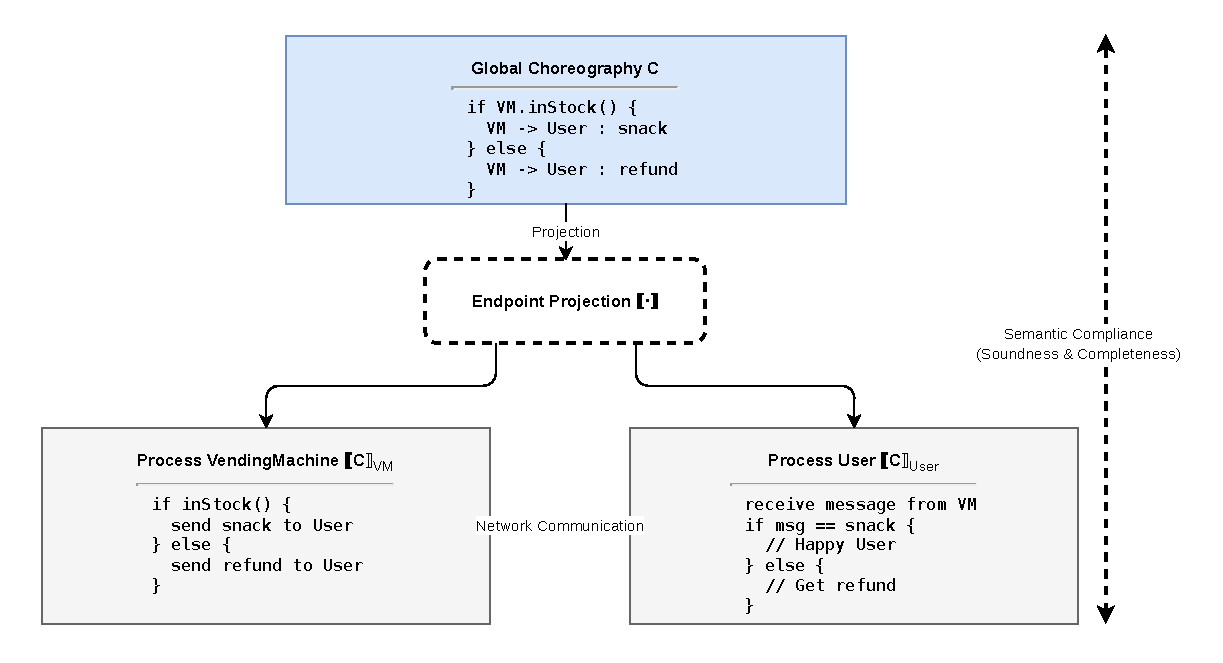
\includegraphics[width=\textwidth]{figures/EPP.drawio.pdf} 
	\caption{Workflow of Endpoint Projection: Decomposing a global choreography $C$ into compliant local terms $\llbracket C \rrbracket_p$.}
	\label{fig:epp_workflow}
\end{figure}

\subsection*{Correctness and Knowledge of Choice}
The central requirement for EPP is \textit{semantic preservation}, which ensures that the generated code faithfully implements the behavior specified in the choreography. This is formally expressed through two properties~\cite{Carbone2012}:
\begin{itemize}
	\item \textbf{Completeness:} The network can perform all transitions defined in the choreography ($C \xrightarrow{\mu} C' \implies \llbracket C \rrbracket \xrightarrow{\mu} \llbracket C' \rrbracket$).
	\item \textbf{Soundness:} The network performs \textit{only} those actions prescribed by the choreography ($\llbracket C \rrbracket \xrightarrow{\mu} N \implies \exists C': C \xrightarrow{\mu} C' \land N = \llbracket C' \rrbracket$).
\end{itemize}
Here, $\mu$ represents a transition label (signifying the interaction or action being performed), while $N$ denotes a network state, i.e., the parallel composition of process terms after a transition.

By satisfying these properties, EPP provides a formal basis for deriving endpoint implementations that are correct by construction and free from communication mismatches, deadlocks, and race conditions under the assumptions of the model. However, a critical challenge remains the \textit{Knowledge of Choice} (KoC) problem: when a choreography contains a conditional branch, the decision (e.g., a local check like \texttt{inStock()}) must be propagated to all affected participants to maintain global consistency~\cite{Montesi2023}. EPP therefore constitutes the central mechanism that connects global choreographic specifications to local distributed behavior and provides the deterministic foundation for the extensions considered in the following chapters.


\section{Markov Chains}
To quantitatively analyze the behavior of distributed systems under uncertainty -- such as communication delays, packet losses, or randomized algorithms -- purely deterministic models are insufficient. Instead, this thesis utilizes Markov chains as a mathematical foundation. A Markov chain is a stochastic process that satisfies the Markov property (memorylessness): the probability of transitioning to a future state depends solely on the current state and not on the history of previously visited states~\cite{Norris1997MarkovChains}. 

In the context of probabilistic model checking and tools such as PRISM, two primary variants are distinguished: $(i)$ Discrete-Time Markov Chains (DTMCs) and $(ii)$ Continuous-Time Markov Chains (CTMCs).

\subsection*{Discrete-Time Markov Chains}
Discrete-Time Markov Chains (DTMCs) model systems where transitions occur in discrete steps. They are particularly suitable for representing randomized algorithms or protocols where time is divided into fixed slots. 

Formally, a DTMC~\cite{Baier2008Principles} is defined as a tuple $\mathcal{D} = (S, s_{\mathit{init}}, P, L)$ where: 
\begin{itemize}
	\item $S$ is a finite set of states;
	\item $s_{\mathit{init}} \in S$ is the initial state;
	\item $P: S \times S \rightarrow [0, 1]$ is the transition probability matrix, such that $\sum_{s' \in S} P(s, s') = 1$ for all $s \in S$;
	\item $L: S \rightarrow 2^{AP}$ is a labeling function that assigns a set of atomic propositions ($AP$) to each state.
\end{itemize}

\paragraph{Example.}
As a simple example, consider a message transmission attempt. From an initial state $s_0$, the system moves to a success state $s_1$ with probability $0.9$ and to a failure state $s_2$ with probability $0.1$. The states $s_1$ and $s_2$ may be modeled as absorbing states, i.e., once reached, the system remains in them with probability 1. Formally, for the state order $(s_{0}, s_{1}, s_{2})$, the DTMC is given by the transition matrix
\[
P =
\begin{pmatrix}
	0 & 0.9 & 0.1 \\
	0 & 1   & 0   \\
	0 & 0   & 1
\end{pmatrix}.
\]

This illustrates the characteristic feature of a DTMC: the next state is chosen according to a discrete probability distribution over successor states.

In the context of this thesis, DTMCs serve as the semantic foundation to model the operational behavior of probabilistic choreographies. Within this framework, states represent global system configurations, while transitions capture atomic execution steps, such as message exchanges or probabilistic branching decisions. The transition probabilities are directly induced by the weights assigned to probabilistic choices within the choreographic specification. Consequently, DTMCs provide a rigorous basis for the quantitative analysis of protocols characterized by discrete-time behavior, such as the Peer-to-Peer protocol (\cref{sec:p2p}) and the Dining Cryptographers protocol (\cref{sec:dining-cryptographers}).


\subsection*{Continuous-Time Markov Chains}
While DTMCs are suitable for discrete steps, many distributed systems exhibit behavior that depends on continuous time, such as communication latencies or hardware failure rates. For these scenarios, Continuous-Time Markov Chains (CTMCs) are employed. 

A CTMC~\cite{Baier2008Principles} is formally defined as a tuple 
$\mathcal{C} = (S, s_{\mathit{init}}, R, L)$, where $S$, $s_{\mathit{init}}$, and $L$ are defined as in a DTMC, but:
\begin{itemize}
	\item $R: S \times S \rightarrow \mathbb{R}_{\ge 0}$ is the transition rate matrix.
\end{itemize}
The time spent in a state $s$ before a transition occurs follows an exponential distribution with the rate $E(s) = \sum_{s' \in S} R(s, s')$.

\paragraph{Example.}
As a simple example, consider a server that alternates between being idle and processing requests. Let $s_0$ denote the idle state, $s_1$ the processing state, and $s_2$ a failure state. From $s_0$, the server starts processing a request with rate $\lambda$. From $s_1$, it either completes the request and returns to $s_0$ with rate $\mu$, or it fails and moves to $s_2$ with rate $\theta$.
For the state order $(s_0, s_1, s_2)$, this yields the rate matrix
\[
R =
\begin{pmatrix}
	0 & \lambda & 0 \\
	\mu & 0 & \theta \\
	0 & 0 & 0
\end{pmatrix}.
\]
This illustrates the defining feature of a CTMC: transitions are governed by rates, which determine how quickly competing events occur in continuous time.

In contrast to DTMCs, CTMCs capture systems whose behavior depends not only on probabilistic branching, but also on the timing of events. This is particularly relevant for modeling real-time aspects of distributed systems, such as communication latencies or stochastic delays. In this thesis, CTMCs are used to analyze time- and performance-related properties, as demonstrated in the evaluation of the Modified Think Team Protocol (\cref{sec:think_team}).

In summary, DTMCs model probabilistic branching in discrete execution steps, whereas CTMCs capture stochastic behavior in continuous time through transition rates.
\section{The PRISM Model Checker}
To evaluate the efficiency and correctness of the choreographic language extension developed in this thesis, the PRISM model checker \cite{Kwiatkowska2018} is used as a primary reference and benchmarking tool. PRISM is a widely established framework for Probabilistic Model Checking (PMC), a formal verification technique used to analyze the likelihood of specific behaviors in stochastic systems. In this work, PRISM serves as a "gold standard" to validate that the state spaces generated by the choreographic projection are mathematically accurate and to provide a baseline for performance comparisons.

PRISM typically operates on high-level system descriptions written in its native PRISM modeling language. This state-based language organizes systems into modules that interact via shared variables and synchronized actions. When a user provides a PRISM model (e.g., a .pm file), the tool performs a process called state-space construction: it explores all possible configurations and transitions to build a global mathematical representation, such as a Discrete-Time Markov Chain (DTMC).

A central part of the evaluation in this thesis (see \Cref{ch:evaluation}) involves comparing the efficiency of this construction process. Specifically, we benchmark the runtime required by PRISM's native compiler to build a model against the time taken by our direct generation approach from choreographic specifications.

While PRISM is primarily used through its high-level language, it also provides an explicit interface for pre-constructed models. This interface allows external tools to bypass the PRISM compiler and provide the transition matrix directly. The explicit representation consists of three primary file formats:
\begin{itemize}
	\item \textbf{States Files (\texttt{.sta}):} An enumeration of all reachable global states.
	\item \textbf{Transitions Files (\texttt{.tra}):} A list of all transitions between states, including their associated probabilities (for DTMCs) or rates (for CTMCs).
	\item \textbf{Labels Files (\texttt{.lab}):} A mapping of states to atomic propositions for property verification.
\end{itemize}

The tool developed in this work is designed to generate these explicit formats directly. This enables a structural validation: by comparing the number of states and transitions in the .sta and .tra files generated by our tool with those generated by PRISM from an equivalent manual model, we can formally verify the correctness of the choreographic projection logic.

Although the core contribution of this thesis is the generation of models, the ultimate purpose of these models is their analysis. PRISM enables the verification of complex properties expressed in temporal logics, such as Probabilistic Computation Tree Logic (PCTL) for DTMCs and Continuous Stochastic Logic (CSL) for CTMCs. These logics allow for the calculation of:
\begin{itemize}
	\item \textit{Probabilities:} ``What is the likelihood that the protocol terminates within $N$ steps?''
	\item \textit{Expected Rewards:} ``What is the expected resource consumption (e.g., energy or time) until termination?''
\end{itemize}
By ensuring that our tool outputs PRISM-compatible explicit files, we provide a seamless path for users to utilize PRISM’s powerful numerical solvers for the downstream verification of generated choreographies.



\chapter{Choreography Language}
\label{ch:choreography_language}
The purpose of this chapter is to formalize the syntax and semantics of the choreography language considered within the scope of this thesis. For the sake of clarity and mathematical tractability, we adopt a process-algebraic format, which makes the notation more concise and better suited for formal definitions, structural induction, and correctness proofs. This abstract representation departs slightly from the concrete syntax implemented in our tool, allowing us to focus on the underlying coordination logic and its direct mapping to probabilistic state-and-transition models.

This formalization builds upon the core framework of ChoreoPRISM, as introduced by Carbone and Veschetti \cite{CarboneVeschetti}. While we maintain the fundamental principle of global coordination, our model introduces significant extensions to handle unbalanced control flows and independent probabilistic branching. These features allow for a more flexible description of distributed protocols while enabling a direct mapping to the state-and-transition representation required for Markov chain generation.

In the following sections, we first define the abstract syntax of the language, followed by an operational semantics that describes how a choreography evolves alongside the system's global state. (Finally, we demonstrate how this semantic model serves as the basis for the automated generation of PRISM-compatible explicit models.)


\section{Syntax}
\label{sec:formal_syntax}
The abstract syntax of the choreography language is formally defined using the Backus-Naur Form (BNF).

Let $p, q$ range over a set of participants $\mathcal{P}$, $x$ over a set of variables $\textit{Var}$, and $v$ over a set of values $\textit{Val}$. 

The core components of the language, choreographies $C$, are defined as follows:

\begin{equation}
	\label{eq:grammar}
\begin{array}{r c l l}
	C & ::= & p \to \{p_1, \dots, p_n\} : \sum_{j \in J} \lambda_j : u_j ; C_j & \textnormal{(Interaction)} \\
	& |   & \textnormal{if } E@p \textnormal{ then } C_1 \textnormal{ [else } C_2] & \textnormal{(Conditional)} \\
	& |   & X & \textnormal{(Recursive call)} \\
	& |   & \mathbf{0} & \textnormal{(Inactivity)} \\
	\mathcal{D} & ::= & X \stackrel{\textnormal{def}}{=} C, \mathcal{D} \mid \emptyset & \textnormal{(Definitions)} \\
	u & ::= & (x' = E) \,\&\, u \mid (x' = E) & \textnormal{(Assignments)} \\
	E, g & ::= & f(\tilde{E}) \mid x \mid v & \textnormal{(Expressions)}
	\end{array}
\end{equation}



\paragraph{Syntactic Constructs and Extensions}
Building on the foundation of \textcite{CarboneVeschetti}, the syntax is adapted to support the additional requirements of the probabilistic models considered in this work.

\begin{itemize}
	\item \textbf{Probabilistic Interaction:} The interaction term $p \to \{p_1, \dots, p_n\} : \sum_{j \in J} \lambda_j : u_j ; C_j$ describes an interaction initiated by participant $p$ towards a set of receivers. The mapping to Markov Chain transitions is performed by interpreting each index $j \in J$ as a distinct outgoing edge from the current configuration $(S,C)$. Specifically, for every branch $j$, the operational semantics (see \cref{sec:semantics}) defines a transition to a successor configuration $(S[u_{j}],C_{j})$ with an associated label $\lambda_{j}$. The term $u_{j}$ denotes a set of local variable updates or assignments performed by the participants during the interaction. In the generated model, the labels $\lambda_{j}$ are directly mapped to the transition rates for CTMCs or probabilities for DTMCs. This approach realizes the direct generation of the underlying stochastic model, a strategy suggested in \cite{CarboneVeschetti} to improve performance by bypassing intermediate code projection.
	\item \textbf{Unbalanced Conditionals:} A central contribution of this work is the support for unbalanced conditionals. In our syntax, the \texttt{else} branch is optional. If omitted, it is semantically equivalent to the null choreography $\mathbf{0}$. This allows for the modeling of "fire-and-forget" or "trigger-based" logic where certain participants only act if a specific condition is met, without forcing a synchronized alternative path.
	\item \textbf{Assignments and State Updates:} The term $u$ allows for multiple simultaneous state updates using the $\&$ operator. This follows the PRISM notation $x' = E$, indicating that variable $x$ will take the value of expression $E$ in the next state of the generated Markov Chain.
\end{itemize}

\section{Semantics}
\label{sec:semantics}
The semantics is adapted from \cite{CarboneVeschetti} and extended to support probabilistic branching and unbalanced conditionals.

The operational semantics forms the core of this thesis, as it provides a formal specification of the rules governing state transitions in the system. Beyond its theoretical role, the semantics serves as the foundation for the implementation of our compiler (see \cref{ch:implementaion}). By directly reflecting these formal rules, the tool systematically explores the state space of a choreography and derives the corresponding transitions of the generated Markov chain in a mathematically sound manner. 

A global state $S$ is defined as a mapping from variables to values: $S : \texttt{Var} \rightarrow \texttt{Val}.$
We define the semantics as the smallest relation 
$\longrightarrow^{\mathcal{D}} \subseteq (S,C) \times \mathds{R} \times (S,C)$. A transition $(S,C) \longrightarrow_{\lambda} (S^{'},C^{'}) $ denotes that the system moves from state $S$ and choreography $C$ to the new state $S^{'}$ and (residual) choreography $C^{'}$ with rate or probability $\lambda$. 

\subsection{Interaction and Branching}
\label{paragraph:interaction}
The (Interact) rule models the synchronous communication between a single sender $p$ and a set of receivers ${p_{1},..., p_{n}}$. In the global view, this interaction is an atomic step, meaning that all involved participants synchronize and transition simultaneously. The branching behavior is inherently stochastic: the interaction offers multiple possible outcomes (branches), indexed by $J$. Each branch $k \in J$ is associated with a specific stochastic value $\lambda_{k}$, which determines the likelihood or timing of that branch being selected. The merge behavior is handled structurally by the continuations $C_{k}$: after the synchronization and the execution of local updates $u_{k}$, the system evolves into the subsequent choreography $C_{k}$. If different branches lead to the same continuation term, they effectively merge in the resulting state space. 

\begin{equation}
	\textbf{(Interact)}~~~
	\frac{k \in J}{(S, p \to \{p_1, \dots, p_n\} : \sum_{j \in J} \lambda_j : u_j ; C_j) \longrightarrow{\lambda_k} (S[u_k], C_k)}
\end{equation}

In this rule, $J$ denotes a finite set of indices representing the possible outcomes of the interaction. For each specific branch $k \in J$, the term $\lambda_{k}$ represents the stochastic parameter of the transition. To ensure a well-defined mapping to Markovian models, we distinguish between two semantics:
\begin{itemize}
	\item In a \textbf{Discrete-Time Markov Chain (DTMC)}, $\lambda_{k}$ denotes a \textbf{transition probability}, where $0 \le \lambda_{k} \le 1$ and the sum of all branch probabilities must satisfy $\sum_{j \in J} \lambda_{j} = 1$.
	\item In a \textbf{Continuous-Time Markov Chain (CTMC)}, $\lambda_{k}$ denotes a \textbf{transition rate}, representing the parameter of the exponential distribution governing the time until the interaction occurs.
\end{itemize}


\subsection{Conditionals and Unbalanced Flows} 
\label{paragraph:conditionals}
Conditionals represent local decision points determined by a specific participant $p$. The (IfThenElse) rule captures deterministic branching based on the evaluation of a local guard $E$ in the current state $S(E\downarrow_{S})$. 

\begin{equation}
	\textbf{(IfThenElse-True)}~~~
	\frac{E \downarrow_S = \textnormal{tt}}{(S, \textnormal{if } E@p \textnormal{ then } C_1 \textnormal{ else } C_2) \longrightarrow_{1} (S, C_1)}
\end{equation}

\begin{equation}
	\textbf{(IfThenElse-False-Balanced)}~~~
	\frac{E \downarrow_S = \textnormal{ff}}{(S, \textnormal{if } E@p \textnormal{ then } C_1 \textnormal{ else } C_2) \longrightarrow_{1} (S, C_2)}
\end{equation}

A significant extension in our framework is the support for unbalanced conditionals, i.e. an \texttt{if}-branch without a corresponding \texttt{else}-branch. This flexibility is crucial for modeling \textit{trigger-based} protocols where certain participants only act if a specific condition is met, without necessitating a synchronized alternative path. Formally, if the guard evaluates to \texttt{false} and no alternative branch exists, the choreography terminates.

\begin{equation}
	\textbf{(IfThenElse-False-Unbalanced)}~~~
	\frac{E \downarrow_S = \textnormal{ff}}{(S, \textnormal{if } E@p \textnormal{ then } C_1) \longrightarrow_{1} (S, \mathbf{0})}
\end{equation}

In this case, the system transitions deterministically to the inactive state $\textbf{0}$, representing the completion of the local execution flow.

\subsection{Recursive Calls}
\label{paragraph:recursion}
To allow for the modeling of repetitive or infinite behaviors -- such as randomized retries, polling loops, or long-running protocols -- the language supports recursion through procedure calls. This mechanism enables a choreography to jump back to a previously defined point in the execution flow.

\begin{equation}
	\textbf{(Call)}~~~
	\frac{X \stackrel{\textnormal{def}}{=} C \in \mathcal{D}}{(S, X) \longrightarrow_{1} (S, C)}
\end{equation}

In this rule $X$ denotes a unique protocol identifier, and $\mathcal{D}$ represents the global set of definitions. The notation $X \stackrel{\textnormal{def}}{=} C$ indicates that the identifier $X$ is formally defined as the choreography $C$ within this set. 

From a semantic perspective the (Call) rule describes the unfolding of the identifier: the system transitions from the call $X$ to its corresponding body $C$ while maintaining the current global state $S$. Since this is a structural step in the control flow, it is treated as a deterministic transition with a weight of $1$. 


\section{Running Example: The \texttt{VendingMachine}}

In \cref{subsec:choreographic_programming_paradigm} we introduced a vending machine protocol as an informal example (see \cref{lst:vending_choreo}) to illustrate the concept of choreographic coordination. We now revisit the scenario using the formal abstract syntax and operational semantics defined in this chapter. 

\begin{listing}[ht]
	\begin{minted}{text}
		{
			Start :=
			if "money < price" @user then {
				["1.0"] "money'=money+1" @user .
				Start
			} else {
				Payout
			}
			
			Payout :=
			if "money >= price" @machine then {
				machine -> user : (
				+ ["0.9"] "snack'=1, money'=0" . END
				+ ["0.1"] "snack'=0, change'=1, money'=0" . END
				)
			}
		}
	\end{minted}
	\caption{A running example: \texttt{VendingMachine}}
	\label{lst:vending_formal}	
\end{listing}


The protocol models the repeated insertion of coins until the required price is reached, followed by a probabilistic payout step. This example demonstrates how recursive calls, conditional branching, and probabilistic interactions are represented in the formal syntax and how they induce a corresponding Markov chain.

The informal protocol can now be expressed in the abstract syntax introduced in \cref{sec:formal_syntax}. The resulting choreography is given in~\cref{lst:vending_formal}. 


Based on the operational semantics defined in \cref{sec:semantics}, the choreography induces a corresponding Markov chain. Each state of the Markov chain is represented as a pair $(S, C)$, where $S$ denotes the valuation of variables and $C$ the remaining choreography.
For illustration, we consider a concrete instance with $price = 2$, resulting in the state space shown in \cref{fig:vending_markov_chain_compact}.

\begin{figure}[ht]
	\centering
	\begin{tikzpicture}[
		>={Stealth[inset=0pt, length=4pt]}, % Kleine Pfeilspitzen
		node distance=2.2cm,               % Etwas kompakterer Abstand
		every node/.style={font=\scriptsize}, 
		state/.style={
			draw,
			circle,                         
			minimum size=1.2cm,             
			inner sep=1pt,
			align=center}
		]
		
		% 0. Der neue Start-Knoten (m=0)
		\node[state] (s0) {
			$C$ \\ 
			$ch=0$ \\ 
			$sn=0$ \\ 
			$m=0$
		};
		
		% 1. Knoten (m=1)
		\node[state] (s1) [right=of s0] {
			$C$ \\ 
			$ch=0$ \\ 
			$sn=0$ \\ 
			$m=1$
		};
		
		% 2. Knoten (m=2)
		\node[state] (s2) [right=of s1] {
			$C$ \\ 
			$ch=0$ \\ 
			$sn=0$\\
			$m=2$
		};
		
		% 3. End-Knoten Snack (m=0, sn=1)
		\node[state] (s3) [right=of s2, yshift=0.85cm, xshift=0.75cm] {
			$C$ \\ 
			$ch=0$ \\ 
			$sn=1$ \\
			$m=0$
		};
		
		% 4. End-Knoten Change (m=0, ch=1)
		\node[state] (s4) [right=of s2, yshift=-0.9cm, xshift=0.75cm] {
			$C$ \\ 
			$ch=1$ \\ 
			$sn=0$\\
			$m=0$
		};
		
		% Transitionen
		\path[->]
		(s0) edge node [above] {1} (s1)
		(s1) edge node [above] {1} (s2)
		(s2) edge [bend left=15] node [above left, pos=0.6] {0.9} (s3)
		(s2) edge [bend right=15] node [below left, pos=0.6] {0.1} (s4);
		
	\end{tikzpicture}
	\caption{Representation of the induced Markov Chain}
	\label{fig:vending_markov_chain_compact}
\end{figure}

To make the connection between the operational semantics and the Markov chain in \cref{fig:vending_markov_chain_compact} explicit, we sketch the derivation of the first transitions for the concrete instance with $price = 2$. Let the initial valuation be
\[
S_0 = \{ money \mapsto 0,\; snack \mapsto 0,\; change \mapsto 0,\; price \mapsto 2 \}.
\]
The initial configuration is then given by
\[
(S_0,\; Start).
\]

Since the guard $money < price$ evaluates to true in $S_0$, the semantics selects the then-branch of the conditional in \texttt{Start}. Executing the assignment
\[
["1.0"]\; money' = money + 1~@user
\]
updates the valuation to
\[
S_1 = \{ money \mapsto 1,\; snack \mapsto 0,\; change \mapsto 0,\; price \mapsto 2 \},
\]
and the recursive call returns control to \texttt{Start}. Hence, one obtains the transition
\[
(S_0,\; Start) \longrightarrow (S_1,\; Start).
\]

Applying the same rule once more yields
\[
(S_1,\; Start) \longrightarrow (S_2,\; Payout),
\]
where
\[
S_2 = \{ money \mapsto 2,\; snack \mapsto 0,\; change \mapsto 0,\; price \mapsto 2 \}.
\]
At this point, the guard $money < price$ is false, so the else-branch is selected, which transfers control to \texttt{Payout}.

In the configuration $(S_2,\; Payout)$, the guard $money \geq price$ evaluates to true, enabling the probabilistic interaction at the machine. According to the semantics of probabilistic branching, this yields two successor configurations:
\[
(S_2,\; Payout) \xrightarrow{0.9} (S_3,\; END)
\qquad\text{and}\qquad
(S_2,\; Payout) \xrightarrow{0.1} (S_4,\; END),
\]
where
\[
S_3 = \{ money \mapsto 0,\; snack \mapsto 1,\; change \mapsto 0,\; price \mapsto 2 \}
\]
and
\[
S_4 = \{ money \mapsto 0,\; snack \mapsto 0,\; change \mapsto 1,\; price \mapsto 2 \}.
\]

These derivation steps correspond directly to the states and transitions shown in \cref{fig:vending_markov_chain_compact}: the first two transitions are deterministic and therefore labeled with probability $1$, whereas the final payout step induces the probabilistic branching with probabilities $0.9$ and $0.1$.



\chapter{Implementation}
\label{ch:implementaion}
This chapter describes how we realized the formal framework developed in \cref{ch:choreography_language} into an executable prototype. To this end, we present \textsc{ARIA}\footnote{The complete source code of \textsc{ARIA} is available at: \url{https://github.com/JTuerker/ARIA}} (Automated Reasoning for Interactive Choreographies), a tool that systematically explores choreographic executions and derives the corresponding Markov chain in an automated and efficient manner.

\section{Goal of the Implementation}
The goal of the implementation is to make the formal framework established in \cref{ch:choreography_language} practically usable. While the theoretical model shows that choreographies give rise to Markov chains, applying this construction to realistic systems requires an automated exploration procedure that can systematically capture large and complex state spaces.
We address this challenge with \textsc{ARIA} by providing an automated pipeline from high-level choreographic specifications to stochastic models.

Specifically, we designed the implementation to achieve the following four objectives:

\begin{enumerate}
	\item \textbf{Automated State-Space Exploration:} We aim to explore all reachable configurations $(S,C)$ of a choreography in a systematic manner. To this end, we implemented the operational semantics using a worklist-based exploration algorithm, which allows us to construct the reachable state space automatically.
	
	\item \textbf{Direct Model Generation:} We focus on the direct construction of the state-space from the operational semantics. By generating states and transitions without relying on an intermediate high-level modeling language, we ensure a precise mapping between our formal model and the resulting stochastic process. This approach allows us to avoid the overhead of an additional compilation step and the necessity of encoding complex, unbalanced control flow into the restricted syntax of guarded command languages.
	
	\item \textbf{Semantic Fidelity:} We ensure that the implementation remains closely aligned with the formal semantics. We designed \textsc{ARIA} such that each generated transition corresponds to a valid application of the inference rules defined in \cref{sec:semantics}. This ensures that the deadlock-freedom-by-design guarantees of our model are preserved in the generated output.
	
	\item \textbf{Interoperability and Validation:} Finally, we ensure that the generated model is fully compatible with established verification tools. We achieve this by exporting the state space into the PRISM explicit format, specifically using the \texttt{.sta} (state) and \texttt{.tra} (transition) file extensions. This interoperability allows us to use \textsc{ARIA} as a specialized front-end for choreographies while leveraging the PRISM model checker for the subsequent analysis and validation.
\end{enumerate}

\section{System Architecture}
We implemented \textsc{ARIA} as a standalone Java application. Its architecture follows a staged pipeline consisting of a \textit{front-end} for choreography processing, a \textit{back-end} for state-space exploration, and a \textit{post-processing} step for serialization to model-checker formats. Java was chosen as the implementation language because it offers a practical balance between portability, type safety, and performance for a compiler-like analysis tool. The project is managed with \textsc{Maven} to support consistent dependency management and reproducible builds.

For the \textit{front-end}, we utilize \textsc{ANTLR4}~\cite{antlr4} as a parser generator to process choreography specifications. Based on the context-free grammar provided by Carbone and Veschetti~\cite{CarboneVeschetti} (see \cref{sec:grammar}), we employ \textsc{ANTLR4} to generate the lexer and parser. We then recursively traverse the resulting parse tree with a custom visitor to construct an Abstract Syntax Tree (AST). This AST serves as our internal representation of the input choreography for the subsequent state-space exploration. 

The back-end of ARIA is centered around a worklist-based state-space exploration engine. We chose an iterative approach over a recursive implementation for two reasons. First, it avoids Java’s call-stack limitations when exploring deep state spaces. Second, it decouples successor generation from the exploration order, allowing the scheduling policy to be varied independently of the semantic rules.
This design proved essential for handling state-space explosion. The iterative worklist-based design decouples successor generation from the exploration order. This flexibility allows the engine to employ a \textit{biased hybrid search strategy}, which can be tuned to balance between different traversal policies depending on the model's complexity (see \cref{sec:efficiency}).

Starting from an initial configuration $(S,C)$, the exploration engine incrementally computes successor states by applying the operational semantics defined in \cref{ch:choreography_language}. To avoid redundant exploration and ensure termination, visited configurations are stored in a centralized hash-based data structure for efficient state deduplication. This is essential for explicit-state generation, since the same global configuration may be reached through different concurrent execution paths. To further optimize performance-critical operations, we employ specialized collection classes from the \textsc{FastUtil} library. By using custom hashing strategies and avoiding the overhead of standard boxed collection types, we reduce heap usage and accelerate state lookups, especially for large state vectors where equality must be determined by content rather than object identity.

To interface with probabilistic model checkers, each discovered configuration is assigned a unique numerical identifier. Serialization into the PRISM explicit format (\texttt{.sta} and \texttt{.tra}) is performed as a separate post-processing step after exploration has concluded. This separation ensures that the available memory is primarily dedicated to state-space exploration, without additional overhead from I/O operations and string formatting during the search phase.

Finally, the implementation is maintained in a Git-based version control system in order to support traceability and reproducibility of further development.


\section{Realization of the Theoretical Model}
This section describes the realization of the theoretical model, bridging the gap between formal semantics and technical execution. To provide a coherent guide through the implementation details, we again use the \texttt{VendingMachine} protocol as a running example, this time in a recursive variant that models continuous operation (see \cref{lst:vending-machine-recursive}).

\begin{listing}[h]
	\begin{minted}{text}
		preamble
		"ctmc";
		"const int price = 2;"
		endpreamble;
		
		user -> user : "money=0";
		machine -> machine : "snack=0", "change=0";
		
		{
			Start :=
			if "money < price" @user then {
				["1.0"] "money'=money+1" @user .
				Start
			} else {
				Payout
			}
			
			Payout :=
			if "money >= price" @machine then {
				machine -> user : (
				+ ["0.9"] "snack'=1, money'=0" . Start
				+ ["0.1"] "snack'=0, change'=1, money'=0" . Start
				)
			}
		}
	\end{minted}
\caption{The recursive \texttt{VendingMachine} protocol}
\label{lst:vending-machine-recursive}
\end{listing}
Lines 13 and 14 realize the recursive continuation of the protocol: after completing the \texttt{Payout} phase, both probabilistic outcomes transition back to the \texttt{Start} protocol, allowing the process to re-enter its initial waiting state and handle further user inputs indefinitely. From a technical perspective, this recursive definition implies that the induced state-space representation contains cycles rather than terminating after a single interaction. This provides a critical test case for our compiler: the exploration engine must correctly identify previously visited state vectors and avoid re-expanding them indefinitely. Only then can the exploration terminate once the finite set of reachable states has been exhausted.

To bridge the gap between this textual specification and the automated generation of the states and transitions, the compiler first translates the input protocol into an Abstract Syntax Tree (AST). As shown in \cref{fig:ast-vending-machine}, this hierarchical representation breaks down the high-level syntax into structured components, including the preamble, role definitions, and control-flow nodes.

\begin{figure}[h]
\centering
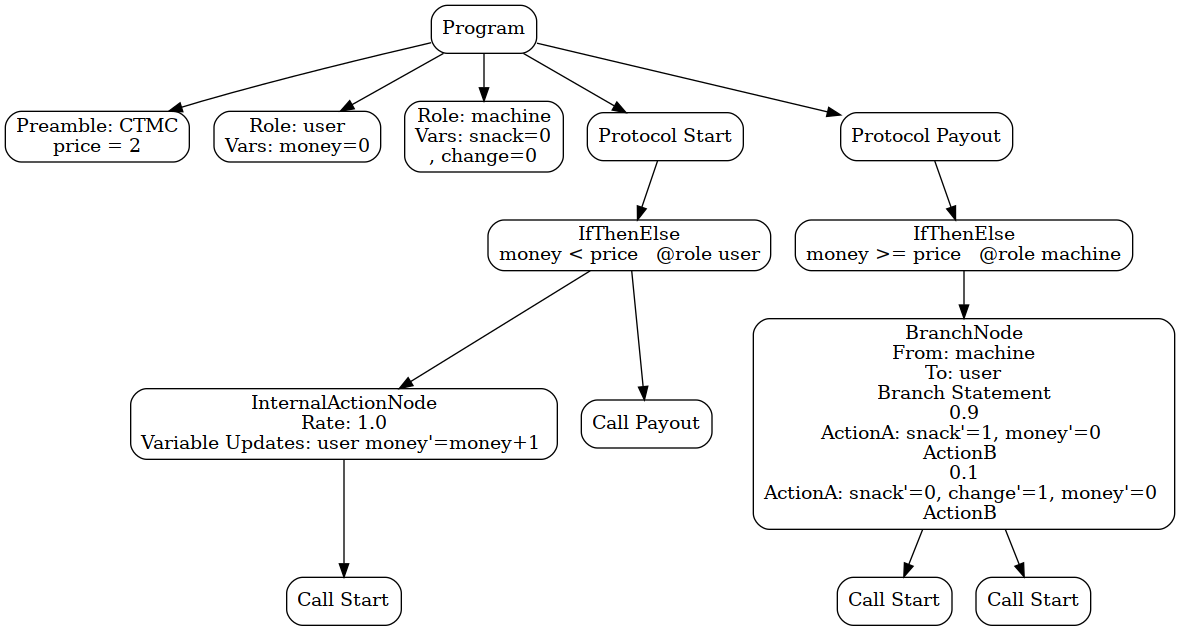
\includegraphics[width=0.9\textwidth]{figures/vendingMachine.png}	
\caption{AST representation of the Vending Machine protocol: each node within the tree is assigned a unique numeric identifier (\texttt{pcId}) during the compilation process. These IDs allow the engine to track the progress of each process by storing the current node's identifier in the program counter segment of the state vector.}
\label{fig:ast-vending-machine}	
\end{figure}
The AST representation is fundamental for the exploration engine: each node within the tree is assigned a unique numeric identifier (\texttt{pcId}) during the compilation process (see \cref{subsec:vector-representation}).
\subsection{State Vector Representation}
\label{subsec:vector-representation}
To manage the state efficiently, we represent the abstract state $S$ as a flat \texttt{Object[]} array in memory. We partition this vector into two distinct logical segments: the \textit{program counter} segment and the \textit{variable} segment. 

The Program Counter (PC) segment stores the current control location for each active process. We manage the mapping of process names to their respective vector indices using the  \texttt{process\-Name\-To\-Pc\-Index} map. During initialization, we define the boundary for the following segment by setting the \texttt{variable\-Section\-Start} offset, which corresponds to the total number of processes in the system (see \cref{lst:pc-mapping}). 
\begin{listing}[h]
\begin{tcolorbox}[
	colback=white,          % Hintergrund weiß
	colframe=gray!50,         % Rahmenfarbe schwarz (oder gray!50 für dezenter)
	arc=0mm,                % Eckige Kanten
	boxrule=0.5pt,          % Dicke der Linie
	left=0mm, right=0mm, top=1mm, bottom=1mm, % Innenabstände der Box
	boxsep=0mm
	]
\inputminted
[linenos, 
firstline=71, 
lastline=72
]{java}{code/MatrixBuilderOnTheFlyWithStateVectors.java}
	
\vspace{-0.7em} \centering \textcolor{gray!60}{$\vdots$} \vspace{0.3em}
 % Block 2: Prozess-Mapping und Segment-Grenze	
\inputminted[
linenos, 
firstline=89,        
lastline=102,         
]{java}{code/MatrixBuilderOnTheFlyWithStateVectors.java}


\vspace{-0.7em} \centering \textcolor{gray!60}{$\vdots$} \vspace{0.3em}

% Block 4: Finale Vektor-Groesse
\inputminted[frame=none, firstline=110, lastline=110]{java}{code/MatrixBuilderOnTheFlyWithStateVectors.java}
\vspace{-0.4em}
\inputminted[frame=none, firstline=111, lastline=111]{java}{code/MatrixBuilderOnTheFlyWithStateVectors.java}
\end{tcolorbox}
\caption{Initialization of the Program Counter mapping}
\label{lst:pc-mapping}
\end{listing}

A key characteristic of our implementation is the dynamic assignment of numeric IDs to AST nodes. Unlike static instruction pointers, these IDs are generated at runtime during each exploration run. Importantly, the IDs do not identify the type of a statement, but its concrete position in the program tree. Thus, even if two syntactically identical statements appear consecutively in the choreography, each receives its own \texttt{pcId}, because they correspond to different locations in the AST.

To support this encoding, we maintain a bidirectional mapping. The \texttt{nodeToPcId} map translates AST node references into numeric identifiers stored in the state vector, while the \texttt{pcIdToNode} list resolves such identifiers back to their corresponding AST nodes during interleaving. In addition, one distinguished ID is reserved for terminal or \texttt{null} states in order to represent process termination. Although the concrete numeric values of the assigned IDs may vary between different executions of the compiler, they remain stable throughout a single exploration run.

\begin{figure}[ht]
	\centering
	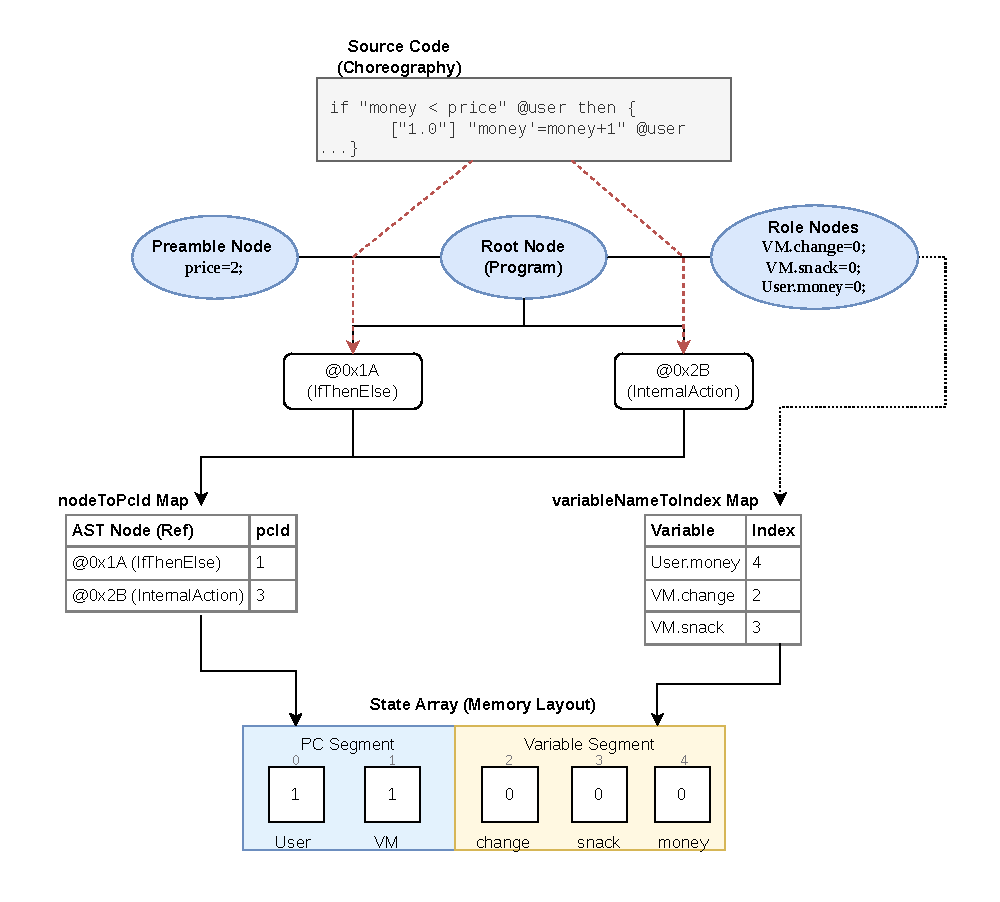
\includegraphics[width=0.9\textwidth]{figures/mapping5.drawio.pdf}
	\caption{Structure of the initial state vector $S_{0}$ for the Vending Machine protocol, illustrating the logical partitioning into the program counter segment and the canonical variable segment.}
	\label{fig:mapping}
\end{figure}


The PC segment is immediately followed by the variable segment, governed by the \texttt{variable\-Name\-To\-Index} map, which provides storage for all global and local variables. To ensure a canonical state representation, which is vital for efficient duplicate detection, we organize the variables lexicographically by their participating role and variable name. This strict ordering ensures that identical system states always result in identical vector representations, regardless of their discovery order.
By determining the \texttt{total\-Vector\-Size} as the sum of the PC indices and the variables upfront, we ensure that the vector's layout remains constant throughout the exploration. As illustrated in \cref{fig:mapping}, this flat structure allows for $O(1)$ access to any part of the system state, which is essential for the high-performance evaluation of guards and the application of assignments during the state space expansion.



\subsection{Stable Node Resolution and Guard Evaluation}
\label{subsec:control-flow}

To optimize the state space exploration, the engine distinguishes between \textit{stable} and \textit{unstable} AST nodes. This distinction is central to our state space reduction strategy. \textit{Unstable nodes} represent administrative or control-flow constructs---such as conditionals (\texttt{IfThenElseNode}) or protocol definitions (\texttt{RecNode})---that do not constitute a distinct, observable state of the distributed system. Instead of materializing these nodes as separate entries in the state space, the engine resolves them internally through a \textit{look-ahead} mechanism.
Execution only halts, and a new state vector is only materialized, upon reaching a \textit{stable node}. Stable nodes correspond to actual behavioral steps, such as communication statements or internal actions. By skipping purely structural transitions and only capturing stable configurations, the engine ensures that the resulting state space remains compact and focuses exclusively on the meaningful interactions and state changes of the choreography.
The core logic of this \emph{look-ahead} mechanism is shown in the simplified \cref{lst:resolve-stable-node}. 

\begin{listing}[h]
\begin{minted}{java}
	function resolveToNextStable(node, state):
		current = node
		while current is unstable:
			if current is Protocol or Recursion:
				current = resolveContinuation(current)
			else if current is If-Then-Else:
				if evaluate(current.guard, state):
					current = current.thenBranch
				else if current.hasElseBranch:
				current = current.elseBranch
				else:
					return null // Blocking Guard
		return current // Found stable action or branch
\end{minted}
\caption{Resolution of unstable AST nodes during state space exploration, including the handling of blocking guards via the \texttt{null} return value.}
\label{lst:resolve-stable-node}
\end{listing}

In the recursive Vending Machine protocol, exploration starts at the \texttt{Start} protocol. At this point, the engine first encounters the guard \texttt{money < price}, represented by an unstable \texttt{If\-Then\-Else\-Node}. Since such nodes only determine the control flow, they do not themselves give rise to a transition. Instead, the guard is evaluated against the current state vector. If the condition holds, the engine continues into the corresponding branch and skips over the unstable control-flow nodes until it reaches the next stable node.

In this example, the next stable node is an \texttt{InternalActionNode} that increments the \texttt{money} variable of the \texttt{user}. This action is only executed if the active process is indeed the \texttt{user}. If another process is currently considered active, the action is not performed. When the role matches, the variable update is applied and the program counter of the active process is advanced to the next control location.

\begin{figure}[h]
\centering
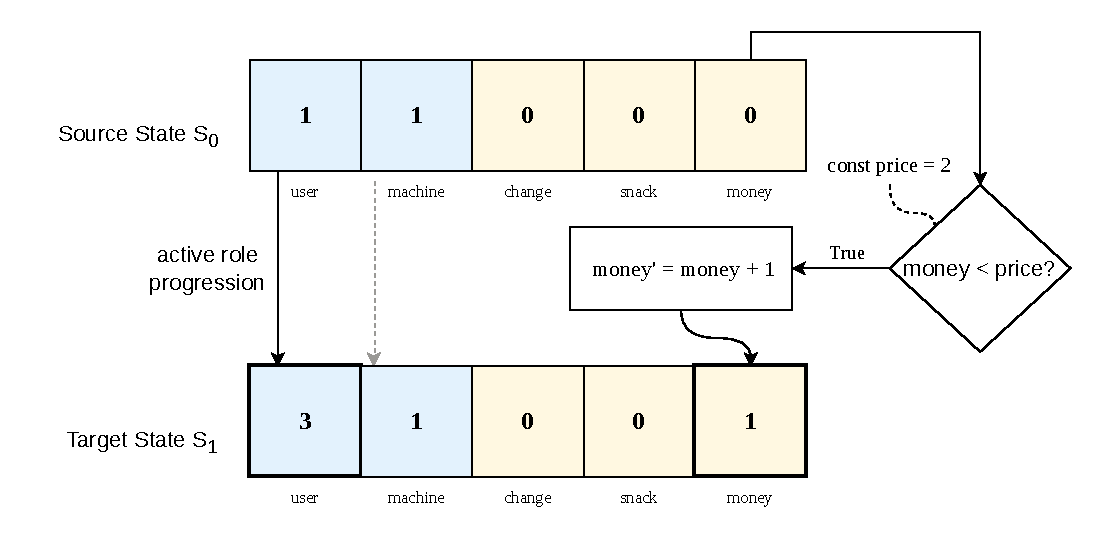
\includegraphics[width=0.9\textwidth]{figures/next_stable.drawio.pdf}
\caption{Atomic transformation of the state vector during a variable update step in the \texttt{Start} protocol. The engine evaluates the guard using the current variable segment and the global constant \texttt{price}. While the active role (\texttt{user}) advances to the next stable node ($\text{ID} 1	\rightarrow 3$) and updates the \texttt{money} variable, the passive role (\texttt{machine}) remains at its previous control location (ID $1$).}
\label{fig:start-protocol}
\end{figure}
As a result, the \texttt{user}'s program counter no longer points to the initial guard location, but to the next resolved position in the AST, namely node 3. The \texttt{machine}, by contrast, remains at node 1, since it has not yet taken part in the current step. In this way, the successor state reflects both the completed internal action of the active process and the unchanged waiting position of the other role.

Once a stable node has been reached, the engine constructs a successor state on a copy of the current state vector. It applies the required variable updates and advances the program counter of the active process to the next resolved location in the AST. The resulting vector is thus a fully formed successor state corresponding to one executable step of the model, rather than a purely intermediate control-flow configuration.

To construct the state transition graph, every discovered successor is passed to the \texttt{TransitionSink} alongside its associated transition rate. This component serves as the 'gatekeeper' of the state space: it performs duplicate detection by checking whether the state vector has already been visited. If the state is new, it is assigned a unique identifier and added to the worklist for further exploration. If the state has been encountered before, the engine simply reuses the existing identifier. By linking the source state to the (new or existing) target state, the \texttt{TransitionSink} incrementally builds the complete system model while ensuring that the exploration remains finite and efficient.

In the presence of recursion, this means that cycles arise when exploration returns to a state vector that is already known. Rather than introducing additional intermediate states for structural recursion steps, the implementation records a transition to the existing state, which makes the cyclic structure directly visible in the state space.

A crucial detail in the \texttt{resolveToNextStableNode} routine is the handling of unbalanced conditionals. If a guard evaluates to \texttt{false} and no \texttt{else} branch is defined, the method returns \texttt{null} (see \cref{lst:resolve-stable-node}). In the context of the state-space exploration, this \texttt{null} value indicates a \emph{blocking guard}: the active process cannot proceed along this execution path in the current state. Consequently, the interleaving engine does not generate any transitions for this process from the given source vector, effectively pruning invalid execution paths and ensuring that the model strictly adheres to the specified synchronization constraints.


\subsection{Synchronized Interaction and Probabilistic Branching}

We realize interactions between roles as synchronized updates of the state vector. When the exploration engine encounters a \texttt{BranchNode}, we identify the designated sender and receiver and check whether both processes are ready to participate in the same interaction. We generate a transition only if the receiver is at a compatible control-flow position. More precisely, the receiver's current program counter must either already point to the same \texttt{BranchNode} or be able to reach it by resolving only unstable nodes, such as \texttt{RecNode}, \texttt{ProtocolNode}, or \texttt{IfThenElseNode}, without executing any intervening stable action.

This alignment of control flows ensures that communication steps preserve the intended handshake semantics of the choreography. In contrast to internal actions, which affect only the active process, a synchronized interaction updates the control locations of both participating roles and may additionally apply the variable assignments associated with the selected branch.

\begin{figure}[ht!]
	\centering
	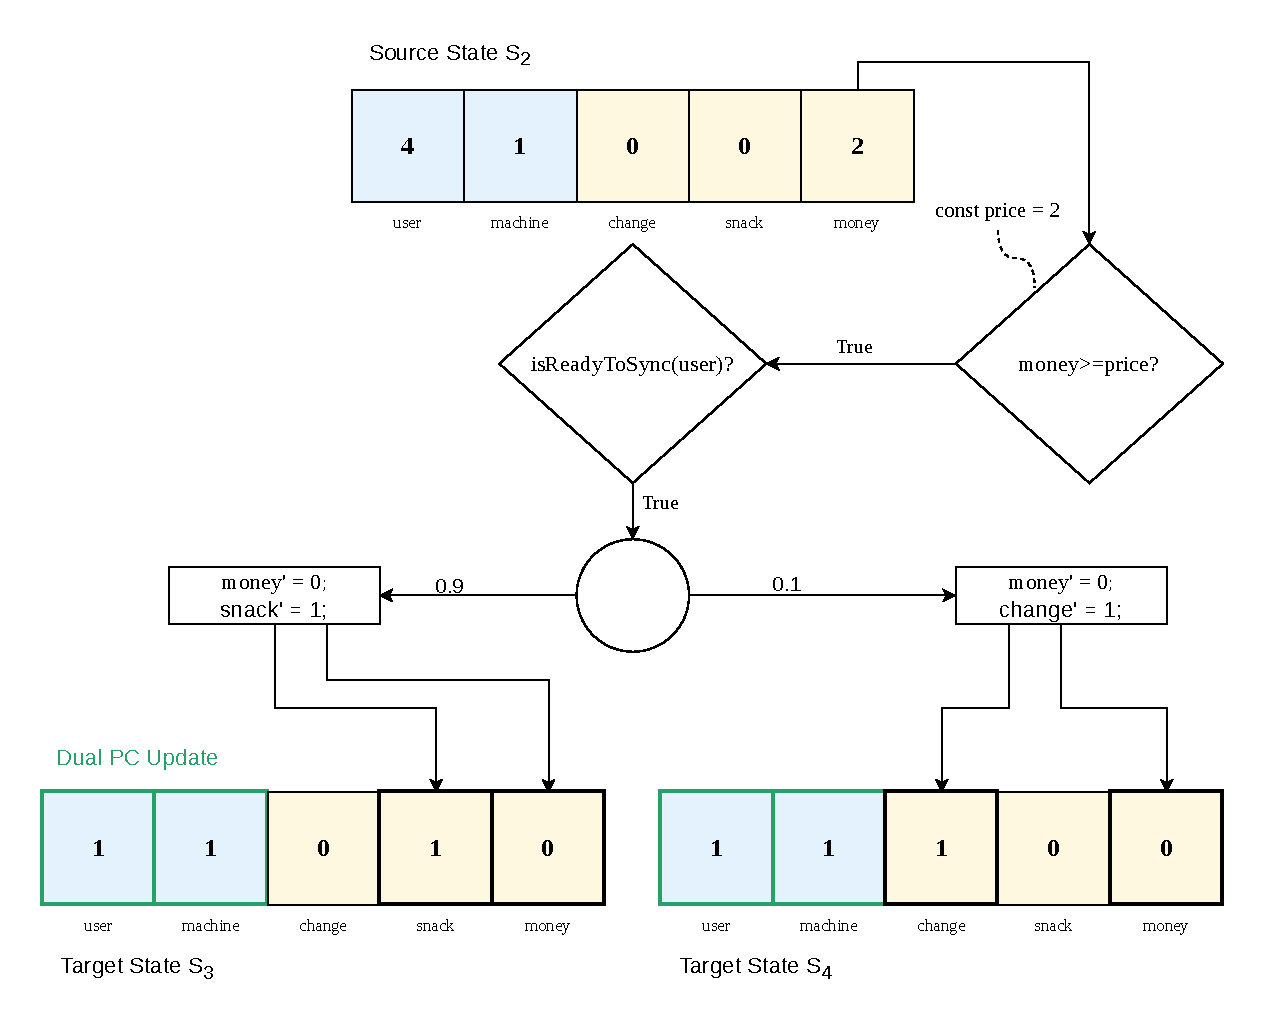
\includegraphics[width=0.95\textwidth]{figures/branching.drawio.pdf}
	\caption{Exploration of a synchronized interaction. Starting from state $S_{2}$	, the engine validates the global guard (\texttt{money >= price}) and the receiver's readiness (\texttt{isReadyToSync}). Upon a successful handshake, the exploration branches into two probabilistic outcomes ($S_{3}|S_{4}$) based on the specified rates (0.9 and 0.1). Each branch triggers a \textit{Dual PC Update} (highlighted in green), where the control locations of both participating roles are updated simultaneously alongside the respective variable assignments.}
	\label{fig:atomic-step}
\end{figure}


In the recursive \texttt{VendingMachine} protocol, this behavior becomes relevant in the \texttt{Payout} phase. We can only realize the communication between \texttt{machine} and \texttt{user} once the accumulated value of \texttt{money} satisfies the guard required to leave the \texttt{Start} phase. Only then can the \texttt{user}'s control flow advance to a position compatible with the \texttt{machine}'s branch, thereby enabling the synchronized interaction.

If this compatibility condition is satisfied, we generate one successor for each probabilistic branch of the interaction (see \cref{fig:atomic-step}). Each successor reflects the selected communication outcome by applying the corresponding assignments and updating the program counters of both roles to their respective continuations. In this way, we represent synchronized communication as a single atomic exploration step in the generated state space.


\subsection{Recursive Control Flow and State-Space Convergence}

We realize recursion by redirecting the program counter (PC) to the entry point of the referenced protocol rather than by introducing stack-based calls. Whenever the exploration reaches a \texttt{RecNode}, the engine resolves the identifier to its corresponding entry point. The program counter of the active process is then reset to the beginning of the respective protocol, ensuring a clean re-entry into the specified control flow.

This mechanism is directly observable in the payout interaction discussed in the previous section. As shown in \cref{fig:atomic-step}, the target states $S_3$ and $S_4$ both feature a program counter of ID 1 for both the \texttt{user} and the \texttt{machine}. This update is the technical result of the recursive call (\texttt{. Start}) at the end of the \texttt{Payout} phase. Instead of pushing a return address to a stack, the engine's routine to resolve continuations (\texttt{resolve\-Continuation}) identifies ID 1 as the stable entry point of the \texttt{Start} protocol and performs a direct PC-substitution. This approach is sufficient because recursion in our choreographic language does not function as a classical subroutine call that requires returning to a caller's context. Instead, recursive calls represent a transition to a renewed protocol behavior. Since there is no subsequent logic to be executed after a recursion is triggered, there is no need to maintain a call stack or track return addresses.

To ensure convergence for cyclic protocols, we maintain a centralized set of previously discovered state vectors. Before a newly generated successor is explored further, we check whether its vector representation has already been encountered. If it is new, it is inserted into the visited-state set and added to the worklist. Otherwise, the existing state is reused and the corresponding transition closes a cycle in the transition matrix.

This mechanism is essential because recursion may return the control flow to an earlier protocol position without reproducing the same global system state immediately. Even if the program counters assume values that have appeared before, exploration must continue as long as the variable segment differs. For instance, a state in which \texttt{snack = 1} is distinct from an otherwise structurally similar state in which \texttt{snack = 0}. Convergence is therefore reached only when the complete state vector, including both control locations and variable valuations, matches a previously discovered configuration. 

The resulting Discrete-Time Markov Chain (DTMC), shown in \cref{fig:vending-full-markov}, represents the complete state space of the Vending Machine protocol. To improve readability, the states are color-coded according to their logical role within the protocol. The grey nodes (0--2) denote the initial synchronization and setup phase that is shared by all execution paths. The blue and yellow clusters distinguish different behavioral branches of the choreography, in particular the \textit{Payout} and \textit{Refund} routines. Probabilistic branching points are highlighted by green edges, which correspond to the stochastic choices specified in the ARIA model, such as the 0.9/0.1 distribution used to represent the payout probabilities. Blue edges indicate recursive transitions. These cycles show that the exploration engine is able to close the state space by returning to previously discovered configurations via direct program-counter substitution, thereby yielding a finite exploration despite the recursive structure of the protocol.
The corresponding \texttt{.sta} and \texttt{.tra} files are provided in the \cref{sec:tra-sta-vending-machine}.

\begin{figure}[ht!]
	\centering
	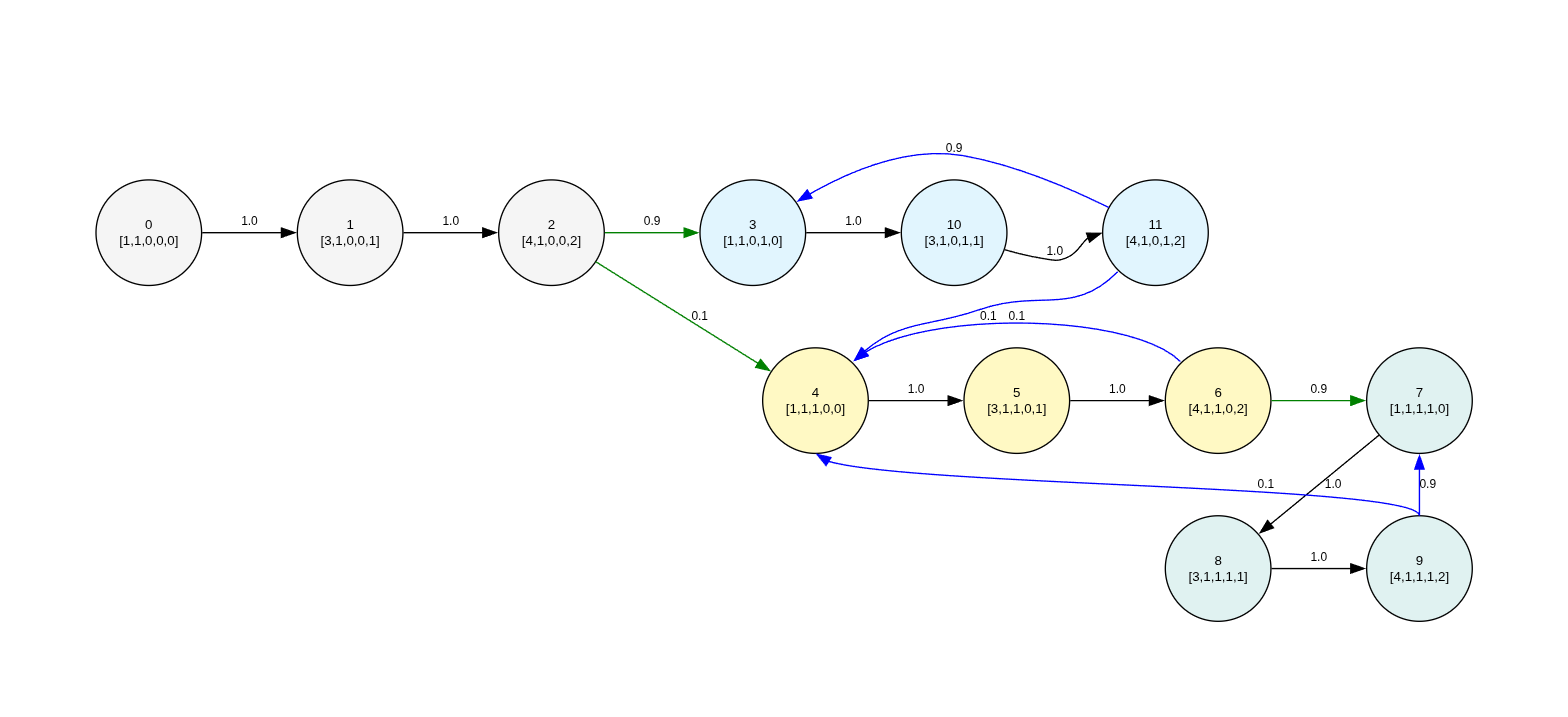
\includegraphics[width=0.95\textwidth]{figures/markovChain.png}
	\caption{Induced Markov chain of the recursive Vending Machine protocol}
	\label{fig:vending-full-markov}
\end{figure}


\section{Challenges}
\label{sec:challenges}
While the formal semantics define which states and transitions must be generated, an efficient implementation also depends on how these structures are stored, traversed, and serialized. This section therefore discusses two practical challenges that emerged during the implementation of \textsc{ARIA}: the decoupling of transition generation from file output, and the memory-efficient handling of explicit states during exploration.
\subsection{Producer--Consumer Decoupling for Transition Output}

A practical challenge in explicit-state exploration is the mismatch between CPU-bound successor generation and I/O-bound transition serialization. If every discovered transition were written to disk immediately, the exploration engine would repeatedly block on file output, reducing overall throughput.

To avoid this, we decouple exploration and serialization using a producer--consumer architecture. The exploration engine acts as the producer, while a dedicated background thread consumes transition records and writes them to the output file. Communication between both components is realized via a bounded \texttt{LinkedBlockingQueue}.

This design serves two purposes. First, it allows exploration to continue while previously generated transitions are being serialized. Second, the bounded queue limits the amount of buffered output and therefore prevents unbounded memory growth if file output temporarily becomes slower than state-space generation.

To terminate the consumer thread in a controlled manner, we use a sentinel record following the \texttt{POISON\-PILL}~\cite{goetz2006java} pattern. Once exploration is complete and no further transitions remain to be emitted, this special record is inserted into the queue, signaling the consumer to finish processing and close the output stream.


\subsection{Memory Efficiency and State Deduplication}
\label{sec:efficiency}

Since explicit-state exploration is inherently vulnerable to state-space explosion, memory efficiency is a central concern of the implementation. In our setting, each state is represented as an \texttt{Object[]} vector containing both control-flow information and variable valuations.

Initially, we attempted to use standard Java collection types, such as \texttt{HashSet<>}, for state storage. However, this approach was insufficient because Java arrays rely on identity-based hashing and equality by default. Consequently, logically identical states reconstructed at different points during the exploration were treated as distinct instances, causing the deduplication to fail and leading to redundant exploration and rapid memory exhaustion. To resolve this, we implemented a custom hashing strategy that compares vectors by their actual contents rather than by object identity. This ensures that two independently constructed vectors are recognized as the same logical state whenever both their program-counter segment and their variable segment coincide.

Beyond state storage itself, the order of exploration also affects memory consumption. Our starting point was a standard breadth-first search (BFS) strategy. While BFS is ideal for finding shortest paths to a state, it requires the engine to store the entire frontier of the search tree in the worklist. For concurrent choreographies with high branching factors, this "frontier explosion" consumed several gigabytes of RAM before any significant depth was reached.

To keep the worklist size manageable, we moved to a biased hybrid search strategy. The worklist is implemented as an \texttt{ArrayDeque}, which allows us to alternate between depth-first and breadth-first expansion. In practice, we predominantly explore states in a depth-first manner (DFS), while periodically taking breadth-first steps to maintain coverage across different execution paths. This combination provides a pragmatic balance between exploration depth and memory stability. A purely breadth-first traversal may cause the worklist to grow rapidly, whereas a purely depth-first traversal may delay the discovery of relevant alternative behaviors. By combining both strategies, we obtain a more robust exploration order while keeping the active frontier within manageable bounds.


\chapter{Evaluation}
\label{ch:evaluation}
This chapter presents the evaluation of the proposed approach. It first outlines the general evaluation setup and then discusses the selected case studies. For each benchmark, the generated state space and the observed runtime behavior are examined.
\section{Evaluation Setup}
This section describes the general setup of the evaluation. It first discusses the main threats to validity and then outlines the methodology used for the experiments, including the execution environment and measurement procedure.
\subsection{Threats to Validity}
As with any empirical and model-based evaluation, the results presented in this thesis are subject to several threats to validity that may affect their generalizability.

A primary threat is the limited number and representativeness of the evaluated case studies. The evaluation considers only three protocols, namely the Modified ThinkTeam protocol, a Peer-to-Peer protocol, and the Dining Cryptographers protocol. Although these examples were selected to cover relevant characteristics of distributed systems, such as probabilistic behavior, coordination patterns, and race conditions, they represent only a small portion of the broader design space. In particular, other systems may differ substantially in terms of communication topology, synchronization structure, concurrency, cyclic behavior, and overall state-space complexity. As a consequence, the results cannot be assumed to generalize directly to all classes of distributed systems, especially with regard to scalability and performance.

A related threat is selection bias. Since the tool was developed and incrementally refined using these case studies, the implementation may have become partially adapted to their specific characteristics. This creates the risk that the evaluation overestimates the general applicability of the approach.

To mitigate these threats, the selected case studies were chosen to cover different forms of probabilistic distributed behavior and different evaluation concerns, as summarized in \cref{tab:case-study-coverage}. In addition, comparisons with PRISM-generated reference models provide a degree of structural validation. While these measures do not eliminate the limitations discussed above, they increase confidence that the proposed approach is not restricted solely to the concrete examples considered here.

\begin{table}[ht]
	\centering
	\caption{Coverage of evaluation case studies in relation to research objectives.}
	\label{tab:case-study-coverage}
	\newcolumntype{Y}{>{\raggedright\arraybackslash}X} % Verbessertes Spaltenlayout
	\begin{tabularx}{\textwidth}{l Y Y}
		\toprule
		\textbf{Case Study} & \textbf{Key Characteristics Covered} & \textbf{Primary Evaluation Objective} \\
		\midrule
		Modified ThinkTeam & Cyclic control flow, mutual exclusion, and symbolic rate-based interactions. & Validation of recursive state closure and parametric model generation (CTMCs). \\
		\addlinespace
		Peer-to-Peer Protocol & Massively concurrent interleavings and combinatorial state-space explosion. & Scalability "stress test" and structural consistency check against PRISM results. \\
		\addlinespace
		Dining Cryptographers & Unbalanced \texttt{if-then} structures (RQ1) and independent local coin flips (RQ2). & Assessment of semantic resynchronization and complex local branching resolution. \\
		\bottomrule
	\end{tabularx}
\end{table}

\subsection{Methodology}

The evaluation in this thesis follows a model-based and experimental approach. The selected case studies were used to assess whether the implemented translation is able to generate explicit-state Markov chain models from probabilistic choreographies, that is, models in which states and transitions are represented explicitly. In addition, the evaluation examines the structural properties of the resulting state spaces. Depending on the example, this includes characteristics such as the number of states, the number of transitions, and the branching structure of the generated model.

All experiments were conducted on the same virtual machine in order to ensure comparability of runtime measurements. The implementation of \textsc{ARIA} was executed using Java~21 on an x86\_64 virtual machine running Ubuntu 24.04.4 LTS, providing 8 virtual CPUs and 23 GiB of RAM under KVM virtualization. Since runtime measurements can be influenced by hardware and system configuration, these details are reported to support reproducibility and interpretation of the results.

Because the engine is written in Java, runtime measurements may be affected by the behavior of the Java Virtual Machine (JVM), in particular by just-in-time (JIT) compilation and runtime optimizations. To reduce the influence of startup effects, each benchmark was executed ten times before measurements were recorded. These warm-up runs allow frequently executed code paths to be optimized by the JVM, resulting in more stable and representative timing results.

After the warm-up phase, the actual measurement runs were performed. Each benchmark was executed ten times, and the reported runtimes correspond to the average over these runs. This helps reduce distortion caused by class loading, interpretation overhead, and initial JIT compilation. In general, the measurements include the I/O overhead incurred by writing the generated model data to disk, which may influence the observed runtimes. The main exception is the large Peer-to-Peer benchmark with approximately 33 million states, which was measured without output generation, as serializing the full model exceeded the practical memory limits of the evaluation environment.

\section{Case Studies}
The following case studies were selected to evaluate the proposed approach on different classes of probabilistic distributed systems. They cover characteristic phenomena such as race conditions, repeated retries, independent probabilistic choices, and unbalanced conditional flows, thus providing a diverse basis for assessing the generated models. At the same time, they make it possible to examine synchronization patterns that are closely related to the deadlock-freedom concerns motivating the extended choreography framework.

Collectively, the three case studies provide the basis for answering \textit{RQ 3}. By comparing the generated state spaces and transition counts with established results from the PRISM model checker, we assess the structural correctness of the \textsc{ARIA} implementation. Furthermore, the performance measurements across varying model sizes demonstrate the practical feasibility of our direct state-space generation approach.
\subsection{Modified ThinkTeam Protocol}
\label{sec:think_team}
The ThinkTeam Protocol\footnote{https://www.prismmodelchecker.org/casestudies/thinkteam.php} originates from an industrial middleware setting for Product Data Management (PDM) in collaborative CAD environments. Its primary purpose is to manage exclusive access to shared documents through a mechanism called vaulting.

The protocol supports standard operations such as \texttt{checkOut} (locking a file for editing) and \texttt{checkIn} (releasing the file). A defining characteristic of the original ThinkTeam implementation is its retrial-based access control: the system does not utilize a central waiting list or FIFO queue. If a user attempts to check out a file that is currently locked by another participant, the request is denied. The user must then enter a retrial mode, periodically attempting to gain access until the file becomes available.

\paragraph{Benchmark Objective: Competition, Retrial, and Starvation-Prone Behavior}
The ThinkTeam case study is a suitable benchmark for our exploration approach because it combines several characteristics that are challenging for explicit-state generation, including concurrent competition, repeated retrials, and cyclic control flow. These features make it a useful test case for assessing whether the implementation can generate the expected transition structure in a systematic and scalable manner.

In a multi-user setting, competition arises whenever the next system state depends on which participant acquires the shared resource first. In the ThinkTeam protocol, this situation occurs whenever a file is released through a \texttt{checkIn} operation. At that point, different classes of users may compete for the lock: users that are already in retrial mode after a failed access attempt, and users that initiate a fresh \texttt{checkOut} request.

This behavior makes the protocol particularly relevant for the present work. It combines probabilistic branching with repeated contention for a shared resource and therefore induces a cyclic transition structure in which starvation-prone behavior can be represented. As a result, the protocol serves as a compact benchmark for evaluating whether the generated state space faithfully captures the interplay between concurrency, retrial behavior, and probabilistic choice.

\paragraph{Choreographic Encoding}
To evaluate the proposed approach, the ThinkTeam protocol was encoded in the extended choreography syntax. Listing~\ref{lst:thinkteam} shows the resulting specification used in the experiments. 

\begin{listing}[ht]
	\begin{minted}{text}
		preamble
		"ctmc";
		"const int n = 3"
		endpreamble;
		
		//Role Definitions
		Checkout ->  Checkout : "c = 0";
		User[i] -> i in [1...n] User[i] : "u[i] = 0";
		
		{
			InitialAccess := Checkout -> User[i] : 
			
				 (+["1 * lambda"] "c'=1" "u[i]'=1" . Success
			    +["1 * lambda"] "c'=1" "u[i]'=2" . RetryPhase)
			
			Success := Checkout -> User[i] : (["1 * mu"] "c'=0" "u[i]'=0" . InitialAccess)
			
			RetryPhase := Checkout -> User[i] : 
			
			     (+["1 * theta"] "c'=1" "u[i]'=1" . Success
			      +["1 * theta"] "c'=1" "u[i]'=2" . RetryPhase)
			
		}
		
		\end{minted}
	\caption{The modified ThinkTeam protocol in the choreography syntax}
	\label{lst:thinkteam}
	\end{listing}
The encoding highlights several key features of the choreographic language used in this thesis. The protocol is expressed through three main recursive procedures, namely \texttt{InitialAccess}, \texttt{Success}, and \texttt{RetryPhase}. The status of the shared document is captured by the variable $c$, where $c = 0$ denotes an unlocked file and $c = 1$ a locked file. The local status of each user $i$ is represented by $u[i]$, where $u[i] = 0$ denotes an idle user, $u[i] = 1$ a user currently holding the file, and $u[i] = 2$ a user in retrial mode. Within this structure, \texttt{InitialAccess} models the first checkout attempt and leads either to \texttt{Success} or to \texttt{RetryPhase}. The \texttt{Success} procedure represents the period of document usage followed by its release via \texttt{checkIn}, whereas \texttt{RetryPhase} captures the repeated competition among users attempting to acquire the lock after a failed access attempt.

By systematically interleaving the actions of all $n$ users, the tool constructs a transition structure with symbolic rate annotations that captures the competition between newly arriving requests and users already waiting in retrial mode.

To provide a clearer understanding of the protocol's cyclic logic, \cref{fig:thinkteam-snippet} shows a simplified state-space snippet for a single user $(n=1)$. While the full state space for larger $n$
(as discussed in \cref{tab:thinkteam_results}) illustrates the scalability of the approach, this reduced view highlights the fundamental transition structure: Black transitions represent initial access attempts ($\lambda$), blue transitions retrial attempts ($\theta$), and green transitions document release ($\mu$). The cyclic structure reflects repeated competition for the shared resource under retrial-based access control.
\begin{figure}
	\centering
	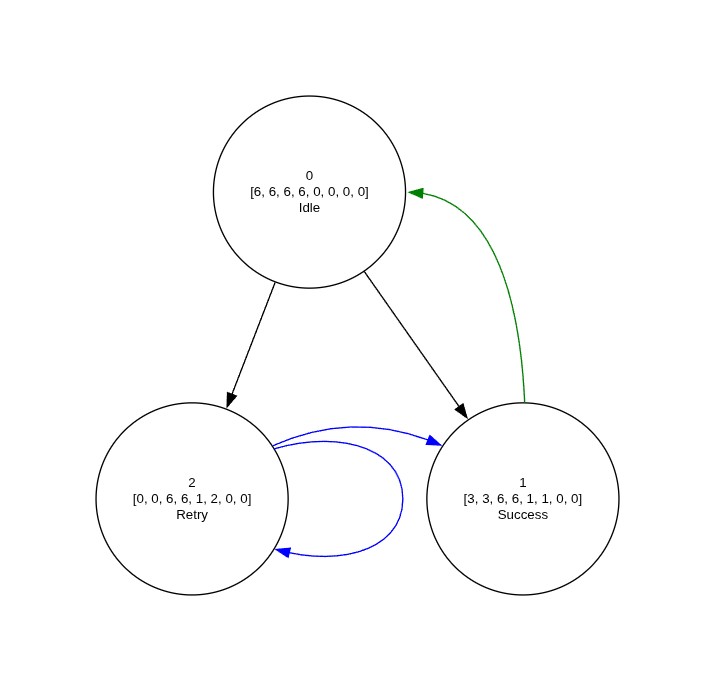
\includegraphics[width=0.75\textwidth]{figures/thinkteam11.png}
	\caption{Generated state space for the modified ThinkTeam protocol}
	\label{fig:thinkteam-snippet}
\end{figure}

\paragraph{Discussion of the Results} 

The experimental results for the Modified ThinkTeam Protocol, shown in Table~\ref{tab:thinkteam_results}, are consistent with the expected behavior of the \textsc{ARIA} exploration engine and provide empirical support for the correctness of the generated state spaces.
\begin{table}[ht]
	\centering
	\caption{Experimental Results for the Modified ThinkTeam Protocol}
	\label{tab:thinkteam_results}
	% Wir definieren einen zentrierten X-Spaltentyp:
	\newcolumntype{Y}{>{\centering\arraybackslash}X}
	
	\begin{tabularx}{\textwidth}{c Y Y Y }
		\toprule
		\textbf{Users ($n$)} & \textbf{States} & \textbf{Transitions} & \textbf{Avg. Time [s]}  \\ 
		\midrule
		1 & 3 & 5  & 0.0047 \\
		2 & 5 & 10 & 0.0049  \\
		3 & 7 & 15 & 0.0052  \\ 
		50 & 101 & 250 & 0.0088\\
		100 & 201 & 500 & 0.0132\\
		500 & 1001 & 2500 & 0.1415 \\
		\bottomrule
	\end{tabularx}
\end{table}

The observed linear growth of the state space ($2n+1$) and the transition count ($5n$) is consistent with the expected theoretical complexity of the protocol. This suggests that the exploration engine handles the interleaving of concurrent request paths in a systematic manner while preserving the intended mutual exclusion behavior of the document vault. The fact that the same structural pattern remains visible even for $n=500$ roles further indicates that the interaction rules scale robustly for this class of examples.

A central challenge in translating choreographies into explicit state spaces is the consistent management of local instruction pointers. The results are consistent with the assumption that \textsc{ARIA} updates the program counters of both the \texttt{Checkout} role and the corresponding \texttt{User[i]} processes coherently during interactions. This includes recursive continuations from \texttt{Success} back to \texttt{InitialAccess} as well as transitions into the \texttt{RetryPhase}. Moreover, the absence of unexpected state growth suggests that no spurious intermediate states are introduced during exploration.

Together, these observations suggest that the generated state space provides a suitable basis for later probabilistic analyses once concrete values are assigned to the symbolic rates $\lambda$, $\theta$, and $\mu$.

The low runtime, including $0.1415$ seconds for 500 users, suggests that for protocols with relatively low coupling, the overhead of exploration remains modest.

\subsection{Peer-to-Peer Protocol}
\label{sec:p2p}

The Peer-to-Peer (P2P)\footnote{https://www.prismmodelchecker.org/casestudies/peer2peer.php} protocol models a decentralized network in which multiple peers exchange data blocks without a central coordinator. From the perspective of state-space exploration, it constitutes a representative example of a highly concurrent system with substantial interleaving and rapid combinatorial growth.

\paragraph{Benchmark Objective: Interleaving, State-Space Explosion, and Emerging I/O Bottlenecks}
In contrast to the modified ThinkTeam protocol, which primarily serves as a compact benchmark for cyclic coordination and retrial behavior, the P2P case study is intended to stress the exploration engine under conditions of extreme concurrency. Its main purpose is therefore to evaluate whether the implementation handles the interleaving of many independently progressing participants correctly and whether it remains robust in the presence of severe state-space explosion.

Due to the large number of peers and the relative independence of their local actions, the protocol induces a very high number of reachable configurations. This makes it a suitable benchmark for testing the correctness of the interleaving logic, the robustness of state deduplication, and the practical scalability of the overall exploration procedure.

At the same time, this case study revealed an additional practical limitation during development and testing. While the exploration itself remained efficient, the explicit serialization of the generated transition structure introduced substantial storage demands. The P2P benchmark therefore also became a useful case for observing how, in large-scale explicit-state generation, the bottleneck may shift from computation to output and storage.

\paragraph{Choreographic Encoding}
As shown in \cref{lst:p2p}, the P2P protocol is encoded using a parametric family of \texttt{Client[i]} roles, where each client maintains a local state describing which data blocks have already been obtained. Concretely, for every client $i \in \{1, \dots, n\}$, the variables \texttt{b[i]1}, \dots, \texttt{b[i]5} record the availability of the corresponding blocks, with value $0$ indicating that a block is not yet available locally and value $1$ indicating that it has been acquired.

The protocol itself is captured by the recursive procedure \texttt{PeerToPeer}. In each execution step, a client performs a local probabilistic action that updates one of its block variables and then recurses back to the same protocol. The five branches shown in the listing correspond to the acquisition of different blocks, each annotated with its own symbolic rate. This encoding abstracts from concrete message-routing details and instead focuses on the stochastic progression of local block acquisition.

From the perspective of state-space exploration, the crucial aspect of this model is that the clients evolve largely independently. Since each \texttt{Client[i]} may perform its next local step without requiring immediate synchronization with the others, the exploration engine must account for a very large number of possible interleavings. Even though the local behavior of an individual client is simple, the combination of parametric roles, recursive continuation, and multiple independently evolving block variables leads to substantial combinatorial growth of the global state space.

This makes the encoding particularly suitable for evaluating whether \textsc{ARIA} can explore large concurrent systems systematically while maintaining a consistent treatment of interleaving and duplicate detection. In this sense, the protocol complements the previous ThinkTeam case study: whereas ThinkTeam emphasizes cyclic coordination and retrial behavior in a comparatively compact state space, the P2P model stresses the exploration engine through massive concurrency and combinatorial growth.

The P2P protocol is the primary benchmark for \textit{RQ 2}. It features a high degree of independence, where multiple peers make local probabilistic decisions about block acquisition. The evaluation focuses on whether the EPP-guided exploration can safely manage the resulting interleavings and the subsequent re-synchronization of these independent local states into a consistent global Markov chain.
\begin{listing}[h]
	\begin{minted}{text}
		preamble
		"ctmc";
		"const int n = 5;"
		endpreamble;
		
		Client[i] -> i in [1...n] Client[i] : "b[i]1 = 0", "b[i]2 = 0" , "b[i]3 = 0", "b[i]4 = 0", "b[i]5 = 0";
		
		{
			PeerToPeer := Client[i] -> Client[i] : 
		   (+["rate1 * 1"] "b[i]1'=1" " " . PeerToPeer
			+["rate2 * 1"] "b[i]2'=1" " " . PeerToPeer
			+["rate3 * 1"] "b[i]3'=1" " " . PeerToPeer
			+["rate4 * 1"] "b[i]4'=1" " " . PeerToPeer
			+["rate5 * 1"] "b[i]5'=1" " " . PeerToPeer)
		}
		
	\end{minted}
	\caption{The Peer-To-Peer Protocol in the specified syntax}
	\label{lst:p2p}
\end{listing}

\paragraph{Discussion of the Results}
\begin{table}[ht]
	\centering
	\begin{threeparttable}
		\caption{Comparison of \textsc{ARIA} and PRISM results for the P2P protocol.}
		\label{tab:p2p_comparison}
		\newcolumntype{Y}{>{\centering\arraybackslash}X}
		
		\begin{tabularx}{\textwidth}{c c Y Y Y Y Y Y}
			\toprule
			\textbf{$n$} & \textbf{$k$} & \textbf{States (ARIA)} & \textbf{States (PRISM)} & \textbf{Transitions (ARIA)} & \textbf{Transitions (PRISM)} & \textbf{Avg. Time [s]} & \textbf{States/s} \\
			\midrule
			4 & 4 & 65{,}536       & 65{,}536       & 1{,}048{,}576   & 524{,}288       & 2.6451   & 24{,}776 \\
			4 & 5 & 1{,}048{,}576  & 1{,}048{,}576  & 20{,}971{,}520  & 10{,}485{,}760  & 46.5617  & 22{,}520 \\
			5 & 4 & 1{,}048{,}576  & 1{,}048{,}576  & 20{,}971{,}520  & 10{,}485{,}760  & 42.6897  & 24{,}564 \\
			5 & 5 & 33{,}554{,}432 & 33{,}554{,}432 & 838{,}860{,}800 & 419{,}430{,}400 & 2343.3567\tnote{*} & 14{,}319 \\
			\bottomrule
		\end{tabularx}
		
		\begin{tablenotes}
			\small
			\item[*] Measured without I/O serialization to disk due to memory limits.
		\end{tablenotes}
	\end{threeparttable}
\end{table}

A comparison with the corresponding PRISM results (see \cref{tab:p2p_comparison}) reveals that the number of reachable states coincides exactly for all evaluated parameter settings. However, the number of transitions generated by \textsc{ARIA} is consistently twice as large as the PRISM count.

This systematic factor of exactly 2.0 is a direct consequence of how self-loops are handled. The state space of the P2P protocol forms a \textit{binary hypercube} of dimension $D = n \times k$, where $n$ denotes the number of peers and $k$ represents the number of data blocks per peer. The total number of reachable states is thus $2^D$. 

In our choreographic encoding (see \cref{lst:p2p}), each peer provides all $k$ acquisition branches in every state. The \textsc{ARIA} exploration engine exhaustively follows every branch defined in the choreography. If a block is not yet possessed, the assignment results in a state change; if the block is already held, the assignment results in a self-loop. Consequently, every state in the \textsc{ARIA} model has exactly $D$ outgoing transitions, leading to a total transition count of $T_{\textsc{ARIA}} = D \cdot 2^D$.

In contrast, PRISM's transition count for CTMCs (specifically in \texttt{.tra} files) typically excludes self-loops, as they do not affect the exit rates or the transient behavior of the Markov chain. PRISM only records the edges of the hypercube where an actual state change occurs. Since a $D$-dimensional binary hypercube has exactly $D \cdot 2^{D-1}$ edges, the resulting ratio is:
\begin{equation}
	\frac{T_{\textsc{ARIA}}}{T_{\text{PRISM}}} = \frac{D \cdot 2^D}{D \cdot 2^{D-1}} = 2
\end{equation}

This observation is important for two reasons. First, the exact agreement in the number of reachable states ($\Delta S = 0$) provides strong empirical support that both tools explore the identical global configuration space. Second, the systematic factor of two indicates that the difference is structural rather than accidental, reflecting a more \textit{semantically exhaustive} representation of the interaction choices in our model. Taken together, these results suggest that \textsc{ARIA} explores interleavings, independent local decisions, and the resulting re-synchronization behavior in a semantically consistent manner.

The measured throughput remains in the range of approximately 22{,}000 to 25{,}000 explored states per second for the smaller configurations and decreases to about 14{,}000 states per second for the largest instance, reflecting the increasing overhead associated with larger state vectors and transition structures.

The declining throughput for larger benchmark instances is consistent with increasing memory pressure during exploration. As the worklist grows and the number of discovered states increases, the implementation must maintain a larger number of live objects simultaneously, including state vectors, worklist entries, and hash-based indexing structures. A plausible consequence is increased heap pressure and additional garbage-collection overhead, which may contribute to the reduced exploration rate. Although no dedicated heap or garbage-collection profiling was performed, the runtime behavior is consistent with this explanation.

For the largest Peer-to-Peer instances, the limiting factor was not only the size of the reachable state space itself, but also the overhead of serializing and storing the generated model. In particular, the output of explicit transition data imposed substantial I/O demands, which became a practical bottleneck alongside memory consumption.
\subsection{Dining Cryptographers Protocol}
\label{sec:dining-cryptographers}

The Dining Cryptographers protocol, originally introduced by Chaum~\cite{Chaum1988}, is a classical benchmark for reasoning about anonymity in distributed systems. The protocol describes a group of cryptographers who wish to determine whether their dinner was paid for by their master or by one of themselves, while preserving the anonymity of the actual payer in the latter case.

The protocol proceeds in two phases. First, each cryptographer flips a private coin and shares its outcome only with the neighbour on the right. Second, each participant announces whether the two visible coin values agree or disagree. If a cryptographer is the payer, however, it announces the opposite result. By evaluating the parity of the public announcements, the group can determine whether the master paid or whether one of the cryptographers paid, without revealing the payer's identity.

\paragraph{Benchmark Objective: Guarded Branching and Conditional Control Flow}
In contrast to the previous case studies, the Dining Cryptographers protocol is particularly useful for evaluating the treatment of conditional control flow. The protocol combines local probabilistic choices with guard-dependent announcements, making it a suitable benchmark for testing whether the exploration engine resolves \texttt{IfThenElse} structures correctly during state-space generation.

Of particular interest is the distinction between balanced and unbalanced conditionals. Depending on the current local observations and on whether a participant is the payer, different control-flow paths become enabled. This makes the protocol well suited for assessing whether the implementation handles both branching cases consistently, excludes blocked continuations correctly from the generated state space, and restores a consistent control-flow alignment when a condition evaluates to false and no explicit \texttt{else} branch is provided.

This protocol specifically addresses \textit{RQ 1}, as it relies heavily on unbalanced conditional flows to model the cryptographers' announcements. It serves as a test case for the semantic rules developed to handle the absence of explicit \texttt{else} branches, ensuring that the exploration engine correctly resynchronizes process control flows even when certain branches are skipped by some participants.

\paragraph{Choreographic Encoding}
In our encoding (see \cref{app:dining-cryptos}), each cryptographer is represented as a separate role with local state variables for the coin value and the final agree/disagree statement. In addition, the model contains a variable identifying the payer. The protocol begins with an initialization step that determines the payer, followed by probabilistic local actions that assign the relevant coin values.

The announcement phase is modeled by guarded transitions whose conditions depend on the local coin value, the neighbouring coin value, and whether the current participant is the payer. As a result, the generated model must combine probabilistic branching, local state updates, and dependency-sensitive guarded control flow in a semantically consistent manner.

For a parameterized system of $N$ cryptographers, the protocol generalizes in the standard way: each participant compares its own coin value with that of its neighbour and publishes either agreement or disagreement, with the payer inverting the expected statement. Collectively, these public announcements determine whether the payer was one of the cryptographers or the master.

\paragraph{Discussion of the Results}
\begin{table}[t]
	\centering
	\caption{Comparison of ARIA and PRISM for the Dining Cryptographers benchmark.}
	\label{tab:dining-comparison}
	\begin{tabularx}{\textwidth}{c|rrr|rrr|rr}
		\hline
		$N$ & \multicolumn{3}{c|}{ARIA} & \multicolumn{3}{c|}{PRISM} & \multicolumn{2}{c}{Difference} \\
		& States & Transitions & Time (s) & States & Transitions & Time (s) & $\Delta S$ & $\Delta T$ \\
		\hline
		3 & 289   & 588    & 0.02999 & 286   & 585    & 0.001 & +3 & +3 \\
		4 & 1736  & 4519   & 0.08096 & 1733  & 4580   & 0.01  & +3 & -61 \\
		5 & 9879  & 32158  & 0.49854 & 9876  & 32315  & 0.03  & +3 & -157 \\
		6 & 54058 & 211185 & 3.21513 & 54055 & 211566 & 0.07  & +3 & -381 \\
		\hline
	\end{tabularx}
\end{table}

\cref{tab:dining-comparison} shows the results of the state-space exploration for the Dining Cryptographers protocol. For all evaluated instances, \textsc{ARIA} constructs exactly three more states than PRISM. This indicates a systematic structural difference between the generated models rather than a random implementation artifact. The number of transitions also differs slightly, although the deviation is not constant across instances: for $N=3$, \textsc{ARIA} generates three additional transitions, whereas for $N \geq 4$ it generates fewer transitions than PRISM.

Overall, the transition counts indicate a systematic but limited discrepancy between the models generated by \textsc{ARIA} and PRISM. In absolute terms, the deviation grows with $N$ ($3$, $61$, $157$, and $381$ transitions for $N=3,\dots,6$), while in relative terms it becomes smaller as the models grow. This suggests that the two constructions remain structurally very close, even though they are not derived from fully equivalent specifications.

A plausible explanation for these differences is that the two models do not encode the protocol in exactly the same way. In particular, the PRISM reference model is formulated as an MDP, whereas the \textsc{ARIA} encoding constructs an explicit state space directly from the choreography. Moreover, the control-flow structure differs slightly: the PRISM model uses local status variables together with explicit enabled commands and a synchronizing \texttt{done} loop, while the choreographic version resolves progress through sequential phases and control-flow resynchronization in the exploration semantics. As a result, both models capture the same protocol behavior at a high level, but they need not induce identical state-transition structures. 

Despite these structural differences, a comparison with established PRISM reference models remains useful for assessing the plausibility of the models generated by \textsc{ARIA}. As widely used representations of the respective protocols, the PRISM models provide a baseline against which the complexity of the generated state spaces can be interpreted. In particular, comparable growth trends as $N$ increases suggest that the choreographic abstraction does not lead to disproportionate additional state-space growth. Such observations do not establish full equivalence, but they do increase confidence that \textsc{ARIA} produces structurally meaningful models that are broadly consistent with established references.


\chapter{Related Work}
\label{ch:related}
This thesis is situated at the intersection of choreographic programming and automated state-space generation for probabilistic verification. In the following, we briefly discuss the most relevant lines of related work and position our contribution with respect to them.

\section{Choreographic Languages and Frameworks}
Montesi’s PhD thesis established key foundations of choreographic programming by introducing a formal model and type theory for the paradigm~\cite{Montesi2013}. As part of this research line, he also presented \textit{Chor}, a prototype framework that supports the development of choreography-based programs together with protocol validation and automatic Endpoint Projection (EPP) to executable Jolie code. By enabling developers to specify communication behavior from a single global perspective and verify it against protocol specifications, this approach supports the construction of distributed software that is safe by construction. Montesi’s later monograph systematizes these ideas and provides a broader overview of choreographic languages and their theoretical foundations~\cite{Montesi2023}. 

Building on these foundations, subsequent work proposed languages and frameworks such as \textit{Choral}~\cite{GiallorenzoMP24}, \textit{HasChor}~\cite{Shen_2023}, and \textit{AIOCJ}~\cite{lmcs:3263}, which explore object-oriented, functional, and adaptive variants of choreographic programming. \textit{Choral} reconstructs choreographic programming through object-oriented abstractions, modelling choreographies as classes and supporting distributed data types, modular composition, and compilation to pure Java libraries. \textit{HasChor}, in contrast, presents a functional formulation in which choreographies are represented as monadic computations in Haskell, with support for higher-order and location-polymorphic choreographies. \textit{AIOCJ} focuses on adaptable distributed applications by allowing designated parts of a choreography to be updated at runtime, while preserving key correctness guarantees such as deadlock freedom and race freedom.

In contrast to existing choreographic programming approaches, which predominantly focus on synthesizing executable distributed implementations from global specifications, this thesis introduced \textsc{ARIA} as a framework centered on formal model construction. Rather than targeting code generation, \textsc{ARIA} supports the automated derivation of analyzable stochastic models from high-level choreographies. In particular, it enables the construction of explicit-state Markov chain models with probabilistic choices and, where applicable, user-provided stochastic parameters. Such models can then be analyzed with probabilistic model checkers such as PRISM in order to study quantitative properties, including performance and reliability. In this way, \textsc{ARIA} extends choreography-based modeling towards quantitative formal analysis.

\section{Model Generation and State-Space Exploration}

Recent work has advanced choreographic programming by mechanizing its theory and compiler infrastructure. Cruz-Filipe et al.\ formalize the paradigm in \textit{Coq} and provide machine-checked proofs of key correctness properties, including deadlock freedom and the correctness of endpoint projection~\cite{cruzfilipe2021}. Building on this line of work, \textit{hacc}~\cite{cruzfilipe2023hacc} is the first certified compiler for a choreographic language, projecting choreographies from a core calculus to an intermediate process representation and ultimately to Jolie code. Similar efforts, such as \textit{Kalas}~\cite{pohjola_et_al2022}, likewise target verified end-to-end compilation from choreographies to executable distributed programs.

While these approaches focus on the translation of choreographic specifications into process code, \textsc{ARIA} considers a different direction, namely the construction of explicit-state stochastic models from choreography semantics. In doing so, it follows an on-the-fly explicit-state exploration paradigm comparable to that used in established model checkers such as SPIN~\cite{Holzmann03} and the explicit-state engine of PRISM~\cite{Prism}. Rather than relying on an intermediate process representation, \textsc{ARIA} explores the global state space by iteratively applying the operational semantics of the probabilistic choreography. This design supports the use of state deduplication and worklist-based traversal techniques during model construction.

\section{Probabilistic Verification of Distributed Systems}

The formal analysis of distributed systems through probabilistic model checking has a long tradition, with tools such as PRISM~\cite{Prism} and Storm~\cite{Storm} representing the current standard for the analysis of Discrete-Time and Continuous-Time Markov Chains (DTMCs and CTMCs). In conventional workflows, however, applying such tools typically requires the manual construction of a system model in a dedicated modeling language, such as the PRISM language. This process is often labor-intensive and error-prone, as it requires the modeller to encode the local behavior of each participant while ensuring that the resulting model correctly reflects the intended global synchronization.

To the best of our knowledge, comparatively less attention has been paid to the automated derivation of stochastic models for quantitative analysis from choreographic specifications. In this context, \textsc{ARIA} explores the construction of explicit-state Markov models from probabilistic choreographies, thereby providing a basis for quantitative formal analysis from a global specification.




\chapter{Conclusion and Future Work}
\label{ch:conclusion}
This thesis introduced \textsc{ARIA}, a framework for the automated generation of stochastic models from choreographic specifications. By extending choreographic programming with probabilistic branching and, where applicable, stochastic parameters, the framework supports the connection between high-level coordination modeling and quantitative formal analysis.

The evaluation based on representative case studies, including the Modified ThinkTeam protocol and Peer-to-Peer models, suggests that \textsc{ARIA} is capable of constructing explicit-state Markov models for non-trivial distributed systems. Comparisons with PRISM-based reference models indicate that the generated models are structurally meaningful and, for selected cases, show a good degree of agreement with established tool-supported results. A central technical contribution of this work is the implementation of an on-the-fly exploration engine that maintains a global state representation while resolving concurrent interleavings and local program-counter updates during model construction.

Overall, the thesis demonstrates that choreographic specifications can serve not only as a basis for correct-by-construction distributed implementations, but also as a starting point for the automated construction of stochastic models for quantitative formal analysis.

While the current prototype of \textsc{ARIA} demonstrates the feasibility of choreography-based stochastic model generation, several directions for future work remain:
\begin{itemize}
	\item \textbf{Expressiveness and Implementation Support:} While the choreographic paradigm itself is highly expressive, the current prototype implementation of the \textsc{ARIA} engine is restricted to a specific subset of the grammar. A natural next step would be to eliminate these implementation-specific limitations by expanding the engine's capability to resolve additional constructs, such as collective synchronization and more generalized guarded command patterns. Supporting a broader fragment of the grammar would bridge the gap between the theoretical framework and the tool's practical expressiveness, enabling the modeling of a wider range of complex distributed protocols.
	
	\item \textbf{Implementation Scalability and Optimization:} The performance analysis of our prototype reveals that for large-scale models, practical bottlenecks are increasingly driven by implementation-specific factors, such as JVM memory management and the high I/O overhead of model serialization. Future work should therefore focus on technical optimizations of the \textsc{ARIA} backend, specifically by investigating more memory-efficient internal data structures and compact binary export formats. Furthermore, the integration of algorithmic reduction techniques---such as partial-order or symmetry reduction---directly into the exploration engine could significantly increase the tool's capacity to handle the state-space explosion in complex distributed systems.
	
	\item \textbf{Formal Semantics and Correctness Guarantees:} Another important direction is the formal study of the semantic relationship between source choreographies and the generated stochastic models. Establishing a bisimulation result, or a similar correspondence between the operational semantics of the choreography and the induced transition system, would strengthen the theoretical foundations of the approach.
	
	\item \textbf{Testing and Validation Infrastructure:} As the framework matures, its implementation could be strengthened through a more systematic testing strategy. Unit tests for core components such as parsing, semantic rule application, and state deduplication could be complemented by integration tests covering the full pipeline from choreography specification to exported model. Such a test suite would improve confidence in future language extensions and help detect regressions during further development.
\end{itemize}

Among the directions outlined above, a formal semantic correspondence between the choreographic source language and the generated stochastic models appears particularly important. While scalability and language expressiveness are relevant for the practical development of \textsc{ARIA}, the broader motivation of choreographic programming lies in the close connection between high-level specifications and their correct realizations. In the context of stochastic model generation, this suggests the need to complement empirical evaluation with a more rigorous formal account of the translation. For example, establishing a bisimulation result, or a similar semantic correspondence, would provide stronger justification that the transitions of the generated Markov model faithfully reflect the coordination behavior described by the source choreography. Such a result would not only strengthen the theoretical foundations of \textsc{ARIA}, but also increase confidence in the quantitative analyses carried out on the generated models.

\printbibliography[heading=bibintoc]

\appendix
\chapter{Appendix}
\label{app:appendix}
\section{Grammar}
\label{sec:grammar}
	\begin{minted}{antlr}
	
	protocol : (preamble)? (varDef)? SEMICOLON (roleDef)+  CLPAR (protocolID ASSIGN blockStatement)* CRPAR ;
	
	protocolID : ID ;
	
	blockStatement : (statement)+;
	
	statement : branch | ifThenElse | end | internalAction | rec;
	
	branch : inputRole=role FROM outputRole+=role (COMMA outputRole+=role)* COLON LPAR (branchStat* | commStat )RPAR ;
	
	branchStat : (BRANCH SLPAR rateValues+=rate SRPAR updates DOT statement) ;
	
	commStat : (SLPAR rateValues+=rate SRPAR updates DOT statement) ;
	
	ifThenElse : IF cond AT role (COMMA cond AT role)* THEN CLPAR thenStat=statement CRPAR (ELSE CLPAR elseStat=statement CRPAR)?;
	
	rec : protocolID ;
	
	end : END (AT CLPAR roles+=role (COMMA roles+=role)* CRPAR)?;
	
	internalAction : SLPAR rate SRPAR message AT role DOT statement;
	
	updates : (SQLPAR (prec=actions) SQRPAR)? upds=message ;
	
	message : actions | first=DOUBLE_STRING loop | loop second=DOUBLE_STRING | loop*;
	
	actions : (action+=DOUBLE_STRING)? ( action+=DOUBLE_STRING)*  ;
	
	loop : FOREACH LPAR indexIteration=index op=(EQ | LE | GE | LEQ | GEQ | NEQ ) upperBound=index RPAR DOUBLE_STRING AT role;
	
	preamble : PREAMBLE (modelType SEMICOLON)? (variableDecl)* ENDPREAMBLE ;
	
	varDef : CHAR EQ INTEGER;
	
	modelType : DOUBLE_STRING;
	
	roleDef : role FROM (indexSpec)? roleSpec* SEMICOLON;
	
	roleSpec : (role (COLON (roleVar (COMMA roleVar)*))?);
	
	roleGroup : ID  ;
	
	roleIndex : ID SLPAR (index | (index BRANCH INTEGER)) SRPAR ;
	
	indexSpec : index IN SLPAR INTEGER DOTS upperBound=CHAR SRPAR ; 
	
	role : (roleGroup | roleIndex) ;
	
	roleVar : DOUBLE_STRING;
	
	variableDecl : DOUBLE_STRING;
	
	rate : DOUBLE_STRING ;
	
	cond : DOUBLE_STRING ; 
	
	index : CHAR ;
	
	SEMICOLON   : ';' ;
	COLON 		: ':' ;
	DOT 		: '.' ;
	DOTS 		: '...' ;
	COMMA		: ',' ;
	BRANCH 		: '+' ;
	FROM 		: '->';
	ASSIGN 		: ':=' ;
	NEQ 		: '!=' ;
	EQ 			: '=' ;
	LEQ			: '<=';
	GEQ			: '>=';
	LE			: '<';
	GE			: '>';
	UNDERSCORE 	: '_' ;
	STAR 		: '*' ;
	LPAR   		: '(' ;
	RPAR   		: ')' ;
	SLPAR   	: '[' ;
	SRPAR   	: ']' ;
	CLPAR  		: '{' ;
		CRPAR  		: '}' ;
	SQLPAR		: '<<' ;
	SQRPAR		: '>>' ;
	AT 			: '@' ;
	IF 			: 'if';
	THEN		: 'then';
	ELSE		: 'else';
	IFplus  	: 'IF' ;
	ELSEplus	: 'ELSE';
	END 		: 'END';
	AND			: '&&' ;
	PREAMBLE	: 'preamble';
	ENDPREAMBLE : 'endpreamble';
	CONST 		: 'const';
	FOREACH		: 'foreach';
	IN			: 'in' ;
	WS  		: [ \t\r\n\u00a0]+ -> skip ;
	DOUBLE_STRING : '"' ~('"')+ '"';
	
	//Numbers
	fragment DIGIT : '0'..'9';    
	INTEGER       : DIGIT+;
	
	//IDs
	CHAR  : 'a'..'z' |'A'..'Z' ;
	ID              :  (CHAR | UNDERSCORE)+ (CHAR | DIGIT | UNDERSCORE | STAR)* CHAR*;
	
	\end{minted}
\captionof{listing}{Grammar for ARIA}
\label{lst:full_grammar}
\newpage
\section{Vending Machine: \texttt{.sta} and \texttt{.tra} files}
\label{sec:tra-sta-vending-machine}
\begin{listing}[h]
	\centering
	\small % Schriftgröße etwas verkleinern, damit es gut nebeneinander passt
	
	% Linke Seite: State Vectors
	\begin{minipage}[t]{0.48\textwidth}
		\centering
		\textbf{State Vectors} \\
		\begin{minted}[fontsize=\footnotesize]{text}
			0: [1, 1, 0, 0, 0]
			1: [3, 1, 0, 0, 1]
			2: [4, 1, 0, 0, 2]
			3: [1, 1, 0, 1, 0]
			4: [1, 1, 1, 0, 0]
			5: [3, 1, 1, 0, 1]
			6: [4, 1, 1, 0, 2]
			7: [1, 1, 1, 1, 0]
			8: [3, 1, 1, 1, 1]
			9: [4, 1, 1, 1, 2]
			10: [3, 1, 0, 1, 1]
			11: [4, 1, 0, 1, 2]
		\end{minted}
	\end{minipage}
	\hfill % Schiebt die beiden minipages auseinander
	% Rechte Seite: Transitions
	\begin{minipage}[t]{0.48\textwidth}
		\centering
		\textbf{Transitions} \\
		\begin{minted}[fontsize=\footnotesize]{text}
			12 16
			0 1 1.0
			1 2 1.0
			2 3 0.9
			2 4 0.1
			3 10 1.0
			4 5 1.0
			5 6 1.0
			6 4 0.1
			6 7 0.9
			7 8 1.0
			8 9 1.0
			9 4 0.1
			9 7 0.9
			10 11 1.0
			11 3 0.9
			11 4 0.1
		\end{minted}
	\end{minipage}
	
	\caption{State vector mapping (\texttt{.sta}, left) and the resulting transition matrix (\texttt{.tra}, right) for the VendingMachine example}
	\label{lst:vending-states-matrix}
\end{listing}
\newpage
\section{The Dining Cryptographers Protocol}
\label{app:dining-cryptos}
\begin{listing}[h!]
	\begin{minted}{text}
		preamble
		"dtmc";
		"const int N = 3;"
		"const int p1 = 1;" "const int p2 = 2;" "const int p3 = 3;"
		endpreamble;
		
		crypt[i] -> i in [1...N] crypt[i] : "coin[i] = 0", "agree[i] = 0", "pay=0";
		
		{InitPay :=
			if "i = 1" @crypt[i] then {
				if "pay = 0" @crypt[i] then {
					crypt[i] -> crypt[i] : (+ ["0.25"] "pay'=0" . Crypto
					+ ["0.25"] "pay'=1" . Crypto
					+ ["0.25"] "pay'=2" . Crypto
					+ ["0.25"] "pay'=3" . Crypto)
				} else { Crypto }
			} else {
				if "pay > 0" @crypt[i] then { Crypto }}	
					
			Crypto := if "coin[i] = 0" @crypt[i]
			then { crypt[i] -> crypt[i] : 
			   (+ ["0.5"] "coin[i]' = 1" . Crypto2
				+ ["0.5"] "coin[i]' = 2" . Crypto2)}
							
			Crypto2 := if "coin[i]>0 && coin[i+1]>0" @crypt[i] then {
				if "coin[i] = coin[i+1]" @crypt[i] then {
					if "pay=p[i]" @crypt[i] then {
						["1.0"] "agree[i]'=0" @crypt[i] . Crypto3     } else {
						["1.0"] "agree[i]'=1" @crypt[i] . Crypto3 }}else {
					if "pay=p[i]" @crypt[i] then {
						["1.0"] "agree[i]'=1" @crypt[i] . Crypto3
					} else {
						["1.0"] "agree[i]'=0" @crypt[i] . Crypto3
			}}}	
		
			Crypto3 := END}		
	\end{minted}
	\caption{The Dining Cryptographers Protocol in the specified syntax}
	\label{lst:dining}
\end{listing}


\chapter{Appendix}
\vspace{2cm}
\section*{Erklärung zur Nutzung von KI-Hilfsmitteln}

Ich erkläre hiermit, dass ich für die Erstellung der vorliegenden Arbeit KI-basierte Werkzeuge zur Unterstützung verwendet habe. 


Die Werkzeuge wurden für folgende Aufgaben eingesetzt: 
\begin{itemize}
	\item Unterstützung bei der sprachlichen Überarbeitung und Korrektur.
	\item Unterstützung bei der Erstellung von Tabellen und Diagrammen
	\item Unterstützung bei der Fehlersuche im Programmcode.
\end{itemize}

Ich bestätige, dass die KI-generierten Inhalte kritisch geprüft, überarbeitet und in die eigene gedankliche Leistung integriert wurden. Die Verantwortung für die Richtigkeit und wissenschaftliche Integrität der Arbeit liegt allein bei mir.

\vspace{1cm}
\noindent Darmstadt, den \today \hfill \rule{5cm}{0.4pt}\\
\phantom{Darmstadt, den \today} \hfill \footnotesize (Unterschrift)



\end{document}
